\documentclass{article}
\usepackage{graphicx}         % For inserting images
\usepackage{amsmath, amsfonts, amsthm}  % AMS packages for math
\usepackage{float}            % For improved figure placement
\usepackage{geometry}         % To customize page dimensions
\geometry{margin=1.25in}
\usepackage{csquotes}         % Context sensitive quotes
\usepackage{url}              % URL formatting
\usepackage{forest}           % For drawing trees
\usepackage{hyperref}         % For hyperlinks
\usepackage{algorithm}        % For pseudocode algorithms
\usepackage{algpseudocode}    % For pseudocode
\usetikzlibrary{quantikz2}    % For Quantum circuit diagrams
\usepackage{tikz}             % For drawing diagrams
\usetikzlibrary{calc, shapes.geometric, arrows, positioning}
\setlength{\parindent}{0cm}
\addtolength{\oddsidemargin}{-2cm}
\addtolength{\evensidemargin}{-2cm}
\setlength{\textwidth}{18cm}
\addtolength{\topmargin}{-2cm}
\setlength{\textheight}{24cm}
\addtolength{\parskip}{5mm}

\title{IFT6135 -- Apprentissage de Représentations (Deep Learning)}
\author{F. Wilhelmy \\
    \texttt{fwilhelmy@hotmail.com}}
\date{Automne 2024}

\begin{document}

\maketitle

\begin{center}
    \huge IFT6135-H25 \\
    \Large Notes du cours -- Hivers 2022 \\
    \vspace{1cm}
    Montreal, QC \\
    \vspace{1cm}
\end{center}
\newpage

%TODOS

% from the standford notes:
    % Weights initialization
    % Also Weight regularization
    % Lagrangian
    % Meta-Learning
    % Main Metrics (Accuracy, Precision, etc...) with confusion matrix
    % beautifull figure for dataset separation
    % neat images for under and over fitting

\section*{Introduction}
These are my personal notes from the course IFT6135 — Representation Learning — taught by Aaron Courville at MILA in Montreal, Quebec, during the Winter 2025 semester. The course ran from January to April, and it was a deep (pun intended) dive into the theory and practice of learning useful representations from data.

That said — fair warning! These notes are incomplete, sometimes messy (I often switch between French and English), and occasionally wrong. They reflect my own understanding of the material, and I’ve tried my best to make sense of complex ideas. Some parts were generated or cleaned up with the help of ChatGPT, others go slightly beyond what was taught in class. There are definitely missing citations, and I still plan to add more figures and references.

I’m sharing these in case they help others going through this intense (but rewarding!) course. If you spot errors, have suggestions, or want to expand a section, feel free to fork the repo and open a pull request. I’ll do my best to review changes promptly. If you do contribute, please don’t forget to add your name to the author list!

A sincere thank you to Professor Aaron Courville for his inspiring lectures, to the TAs for crafting such challenging and thought-provoking assignments, and to all the students — especially Thomas, Maël and Olivier — whose discussions, questions, and collaboration made the learning process far more engaging. It was a real privilege to be part of such a passionate and driven group.

And for those reading this outside the context of MILA — welcome! You’ll probably get the most out of these notes if you already have some background in math, computer science, and deep learning. A solid starting point is the Deep Learning book: \url{https://www.deeplearningbook.org/}.

Enjoy the ride — and good luck with your learning journey!

\newpage

\tableofcontents
\newpage

\section{History} \label{sec:history}

\begin{figure}[ht]
    \centering
    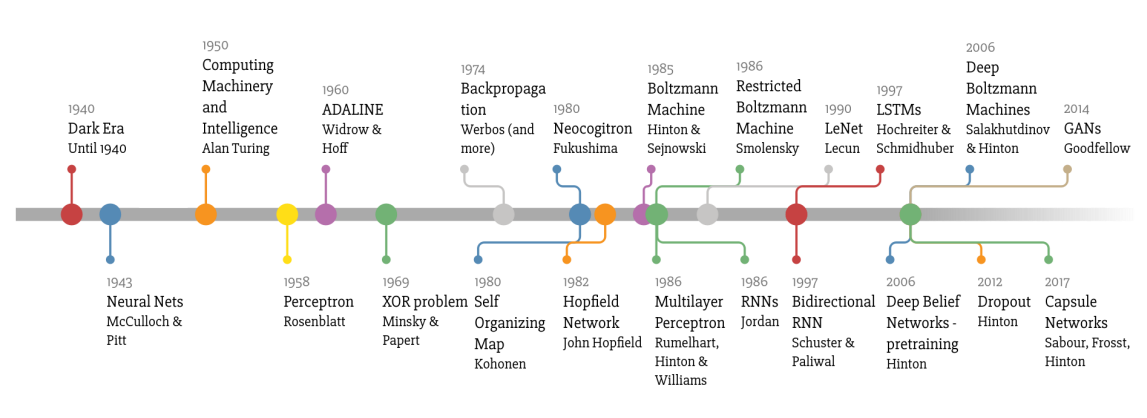
\includegraphics[width=1\linewidth]{graphics/S1History/ai_history.png}
    \caption{Contexte historique}
    \label{fig:ai-history}
\end{figure}

\paragraph{Naissance de l'IA (années 1950)}
Le début du domaine de l'IA (intelligence artificielle) a eu lieu vers 1950.
\begin{itemize}
    \item Perceptron de McCulloch et Pitts (modèle de neurone artificiel).
    \item Apprentissage de Rosenblatt (introduction du calcul de l'erreur).
    \item Théorie du calcul de Turing.
    \item Théorie de l'information de Shannon.
\end{itemize}

Le neurone artificiel est une inspiration de son homologue biologique. Il est composé d'entrées, de poids et d'une fonction d'activation. Initialement, il n'existait pas de mécanisme d'apprentissage. Rosenblatt a introduit un apprentissage basé sur le calcul de l'erreur, mais sans descente de gradient, limitant les réseaux à une seule couche.

\paragraph{Premier hiver de l'IA (années 1960-1970)}
Le problème du XOR soulevé par Minsky et Papert a mis en évidence une limitation majeure du perceptron, menant à un désintérêt général pour l'IA et à une réduction des investissements dans le domaine. C'est à cette époque que les Multi-Layer Perceptrons (MLP) ont été introduits, permettant de dépasser la contrainte de séparabilité linéaire des données. L'introduction de la \textbf{rétropropagation} a marqué une avancée majeure :
\begin{itemize}
    \item \textbf{Efficace} : Complexité de \( O(N) \), où \( N \) est le nombre d'exemples.
    \item \textbf{Générique} : Basé sur la descente de gradient, encore utilisé aujourd'hui.
    \item \textbf{Local} : Aucune garantie de trouver une solution optimale globale.
\end{itemize}

\paragraph{Retour de l'IA (années 1990)}
Dans les années 1990, l'intelligence artificielle a connu un renouveau avec l'apparition de nouveaux modèles :
\begin{itemize}
    \item \textbf{LeNet} de Yann LeCun, utilisé pour la reconnaissance automatique de caractères.
    \item \textbf{Réseaux récurrents} développés par Hochreiter et Schmidhuber, permettant la représentation de séquences.
\end{itemize}

\paragraph{Deuxième hiver de l'IA (années 2000)}
Un nouvel hiver de l'IA est survenu, causé principalement par :
\begin{itemize}
    \item Le problème du \textit{vanishing gradient}, empêchant l'entraînement des réseaux de plus de 3-4 couches.
    \item Le manque de justification théorique des performances des réseaux de neurones.
    \item L'apparition des SVMs (machines à vecteurs de support) qui offraient des performances comparables avec moins de complexité et d'hyper-paramètres.
\end{itemize}

\paragraph{Début de l'apprentissage profond (2006)}
À partir de 2006, des méthodes ont été développées pour entraîner efficacement des réseaux de neurones profonds :
\begin{itemize}
    \item Deep Boltzmann Machines.
    \item Deep Belief Networks.
    \item Pré-entraînement non supervisé et apprentissage par couche.
\end{itemize}
L'entraînement des autoencodeurs par couche était alors fastidieux, nécessitant des sous-entraînements successifs.

\paragraph{Explosion de l'apprentissage profond (2012-2013)}
L'année 2012 marque un tournant majeur avec l'introduction d'AlexNet (SuperVision) lors de la compétition ImageNet. Plusieurs innovations ont contribué à ce succès :
\begin{itemize}
    \item Fonction d'activation \textbf{ReLU}.
    \item \textbf{Augmentation des données} pour améliorer la robustesse des modèles.
    \item \textbf{Réseaux convolutifs} pour extraire des caractéristiques hiérarchiques des images.
    \item \textbf{Utilisation des GPUs}, rendant l'entraînement des modèles plus rapide et efficace.
    \item Accès à de grandes bases de données comme ImageNet.
\end{itemize}

\subsection*{Aujourd'hui}
L'apprentissage profond est omniprésent et trouve des applications variées dans de nombreux domaines.

% =============================================================
\clearpage\newpage

\section{Fundamental Concepts}

\subsection{Définition de l’apprentissage machine}
La programmation 'manuelle' est un processus/algorithme qui a comme entrée des données et des instructions (règles) et qui produit une sortie.

À l'inverse, l'apprentissage machine est un système où l'on fournit en entrée des données et la réponse attendue pour une certaine donnée. La sortie de ce système est un ensemble de règles (modèle) qui cherche à généraliser une relation entre les données et leur sortie respective.

\begin{figure}[ht]
    \centering
    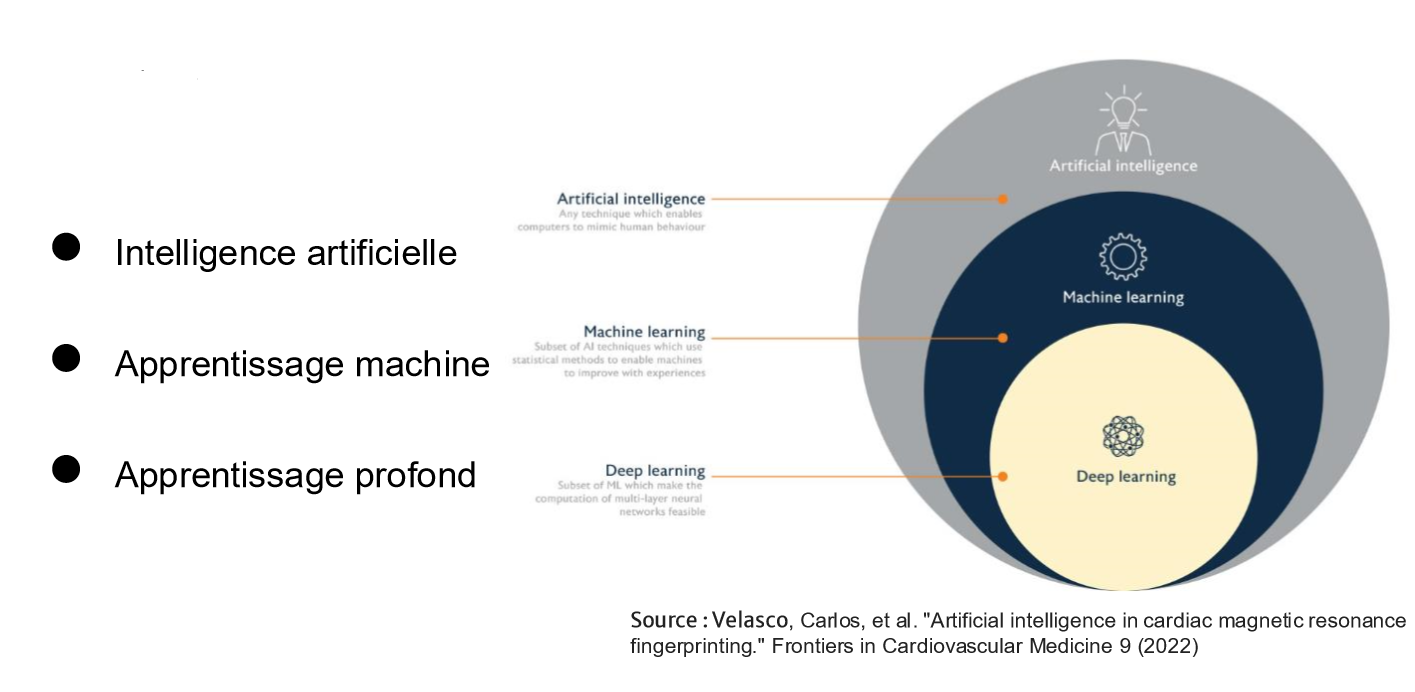
\includegraphics[width=0.5\linewidth]{graphics/S2Intro/AITerms.PNG}
    \caption{Terminologie de l'IA}
    \label{fig:ai-terms}
\end{figure}

\begin{figure}[ht]
    \centering
    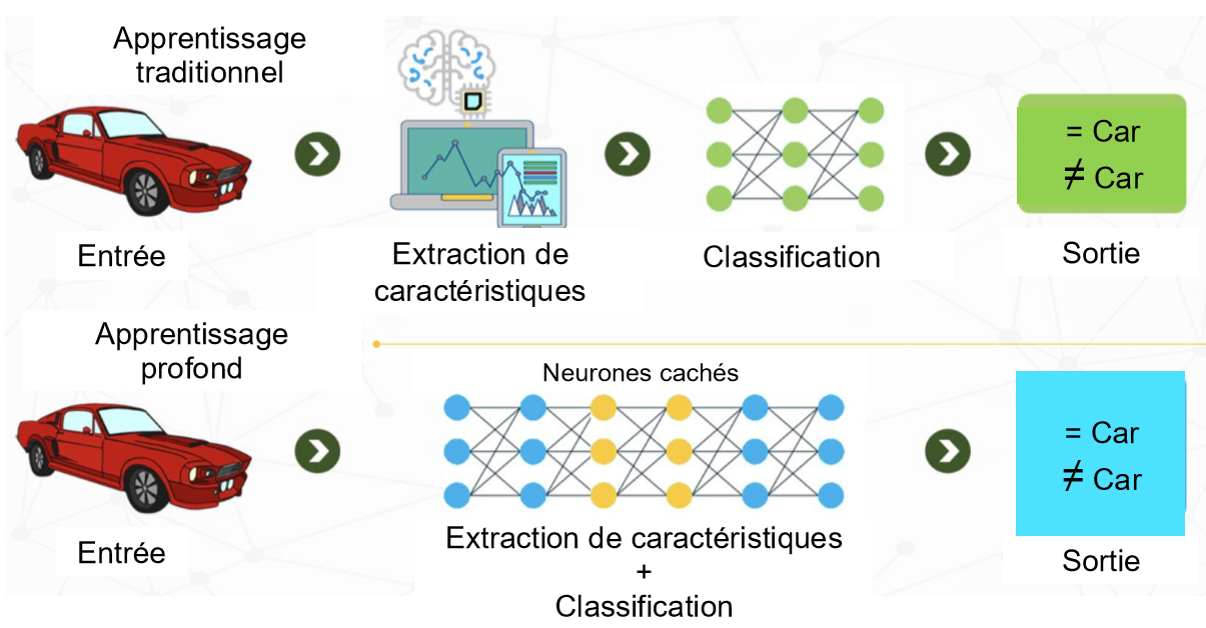
\includegraphics[width=0.7\linewidth]{graphics/S2Intro/ml_vs_dl.PNG}
    \caption{Différence entre l'apprentissage machine et l'apprentissage profond}
    \label{fig:ai-terms-dl}
\end{figure}

\subsection{Le Perceptron}
Le perceptron est le bloc de construction de base dans les réseaux de neurones. Deux composants essentiels :
\begin{enumerate}
    \item \textbf{La somme pondérée (\(net_j\)) :}
    \[
    net_j = \sum_{i=0}^{n} x_i w_{ij} = \vec{w}_j \cdot \vec{x} = \mathbf{w}_j \mathbf{x}
    \]
    ou, en termes du produit scalaire et de l’angle \(\alpha\),
    \[
    net_j = |\mathbf{w}_j| |\mathbf{x}| \cos(\alpha).
    \]
    
    \item \textbf{La fonction d'activation (\(F\)) :} introduit la non-linéarité en activant ou désactivant le neurone selon l’agrégation pondérée des entrées.
\end{enumerate}

\begin{figure}[ht]
    \centering
    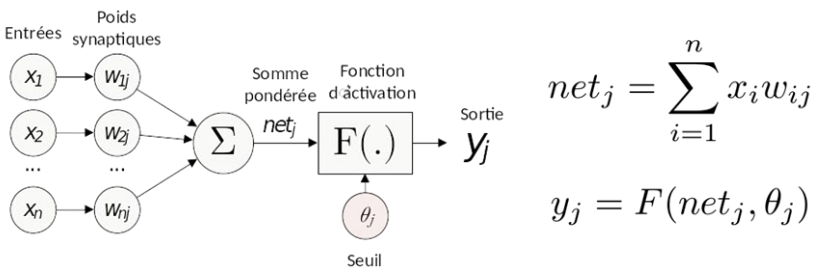
\includegraphics[width=\linewidth]{graphics/S2Intro/perceptron.png}
    \caption{Schéma d’un perceptron}
    \label{fig:perceptron}
\end{figure}

Note importante : Une caractéristique importante du perceptron est qu'il est sensible à l'ordre des données d'entrée. Deux ensembles de données identiques mais présentés dans un ordre différent peuvent produire des ajustements de poids différents.

L'ajustement des poids par la correction de l'erreur a permis au perceptron d'apprendre, mais il n'était pas capable de résoudre certains problèmes comme le problème du XOR. Cette limitation a été surmontée avec l'introduction de méthodes d'optimisation plus avancées, telles que la descente de gradient. Cependant, le choix de la fonction d'activation dans ces méthodes est crucial pour assurer un apprentissage efficace.

\subsection{Neural Networks Layer (NEW)}
In a deep neural network, we can find multiple layers of different functions. The most basic one is a Fully Connected Layer.

For an input of \(N_{in}\) neurons and an output of \(N_{out}\) neurons:
\[
\text{Total Parameters} = N_{in} \times N_{out} + N_{out}.
\]

\subsection{Conception d’un Modèle}
La conception d'un modele d'apprentissage profond peut être décomposée en 4 étapes :
\begin{itemize}
	\item Definition de la taches et du dataset
    \item \textbf{Sélection du modèle}
    \item \textbf{Choix de la fonction de coût}
	\item Optimisation du modele
\end{itemize}

\subsubsection{Le Modèle}
Un modèle efficace doit généraliser et représenter les données. Le choix dépend aussi des contraintes de déploiement (puissance de calcul, rapidité, etc.) et il peut être pertinent de se demander si l'utilisation de l'IA est nécessaire ou si un algorithme plus simple pourrait suffire.

\subsubsection{L’Optimisation}
Cette phase cherche la configuration optimale des paramètres dans l’espace de la fonction de coût. La validation permet d’éviter les problèmes de surapprentissage et de sous-apprentissage.

\begin{figure}[ht]
    \centering
    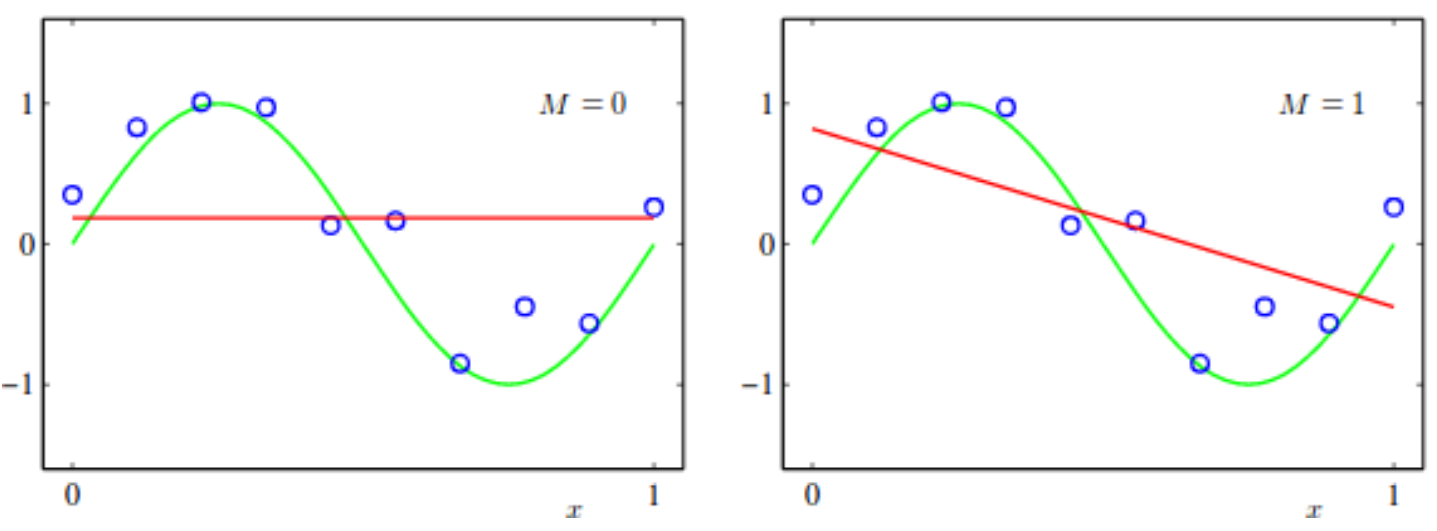
\includegraphics[width=\linewidth]{graphics/S2Intro/sous-apprentissage.PNG}
    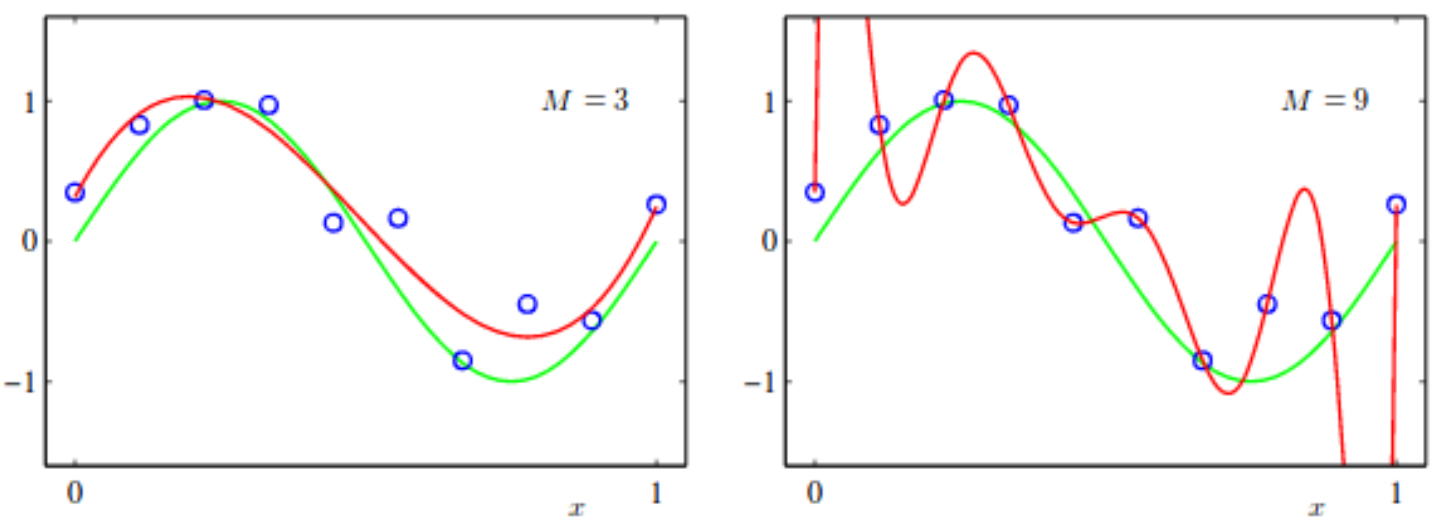
\includegraphics[width=\linewidth]{graphics/S2Intro/sur-apprentissage.PNG}
    \caption{Exemple de surapprentissage (overfit) et de sous-apprentissage (underfit)}
    \label{fig:over-under-fit}
\end{figure}

\subsubsection{Bias-Variance Tradeoff}
The overall error can be decomposed as:
\[
\text{Total Error} = \text{Bias}^2 + \text{Variance} + \sigma^2,
\]
with
\[
\text{Bias}[\tilde{f}] = E[\tilde{f}] - f \quad \text{and} \quad \text{Variance}[\tilde{f}] = E\big[(\tilde{f} - E[\tilde{f}])^2\big].
\]

\begin{figure}[ht]
    \centering
    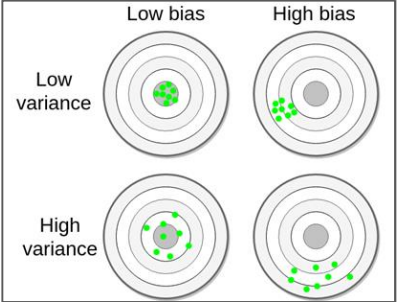
\includegraphics[width=0.7\linewidth]{graphics/S2Intro/biais-variance.png}
    \caption{Bias-Variance Tradeoff}
    \label{fig:biais-variance}
\end{figure}

\subsection{Types de Problèmes}

\begin{itemize}
    \item \textbf{Régression :} \(x \xrightarrow{} \mathbb{R}\)
    \item \textbf{Classification :} \(x \xrightarrow{} \mathbb{N}\)
\end{itemize}

\subsection{Types de Modèles}
Les approches de l'apprentissage machine se classent en différentes familles :
\begin{itemize}
    \item \textbf{Supervisé :} Toutes les données sont étiquetées.
    \item \textbf{Non-supervisé :} Aucune étiquette n’est disponible.
    \item \textbf{Semi-supervisé :} Seule une partie des données est étiquetée.
    \item \textbf{Auto-supervisé :} Des étiquettes peu coûteuses sont générées pour des tâches auxiliaires.
    \item \textbf{Apprentissage par renforcement :}
\end{itemize}

\begin{figure}[ht]
    \centering
    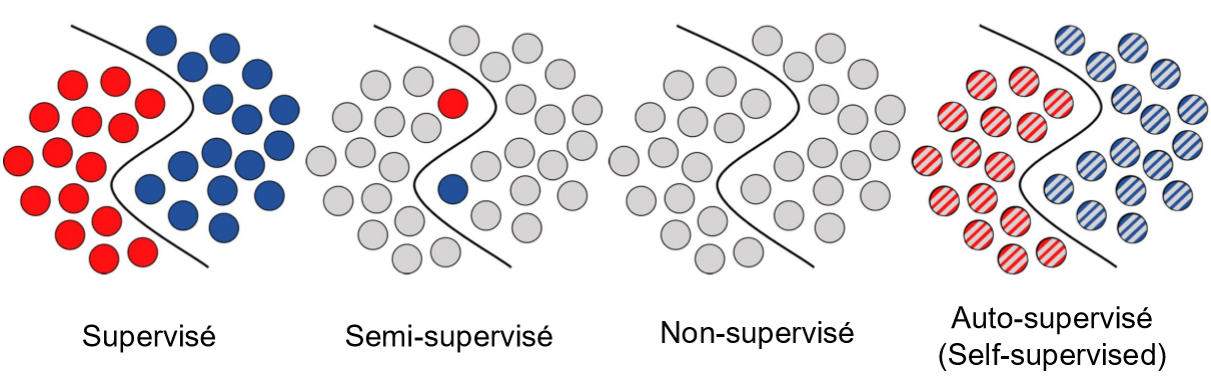
\includegraphics[width=\linewidth]{graphics/S2Intro/learning_type.png}
    \caption{Différents types d’apprentissage}
    \label{fig:learning-types}
\end{figure}

\subsection{Inductive Bias in Machine Learning}
Inductive bias refers to the assumptions a model makes to generalize from training data to unseen data. Different architectures (e.g., CNNs, RNNs, Transformers) incorporate unique biases that affect how they learn and represent information.

Given that real-world data is limited, an inductive bias enables a model to make reasonable predictions by imposing constraints on the possible functions it can learn.

Deep learning architectures have specific biases that give them particular strengths and limitations. For instance, CNNs exploit spatial locality, while Transformers capture long-range dependencies using attention mechanisms.

\begin{itemize}
    \item \textbf{Smoothness Bias}: Similar inputs yield similar outputs.
    \item \textbf{Linear Separability}: Data can be separated by a linear boundary (used in logistic regression and SVMs).
    \item \textbf{Locality Bias}: Local structures are emphasized (as in CNNs).
    \item \textbf{Sequential Dependence}: Past information influences future predictions (as in RNNs).
    \item \textbf{Attention-Based Bias}: Certain input features are weighted more heavily (as in Transformers).
	\item \textbf{Manifold Hypothesis}:
\end{itemize}

Depending on the level of bias imposed on the modele, we get different results.

\begin{itemize}
    \item \textbf{Strong Inductive Bias:} Imposes strong assumptions for faster learning but reduced flexibility (e.g., linear regression).
    \item \textbf{Weak Inductive Bias:} Fewer assumptions allow greater flexibility but require more data (e.g., deep neural networks).
\end{itemize}

% =============================================================
\clearpage\newpage

\section{Optimization Methods} \label{sec:optimization}
Optimization methods search for the best parameter configuration by minimizing the loss function. Generally, optimization techniques will focus on improving the training accuracy of the model and tit's convergeance speed. Asopposed to regularisation techniques (that we will cover lated that are more focused on the ability of the model to generlise . Therefor soetimes slwolying the training. En d'autre mot, elle va determiné si on réussis a trouvé le minimum de notre fonction de cout (loss function).

\begin{itemize}
    \item Evolutionary algorithms.
    \item Closed-form solutions.
    \item Gradient-based methods (first and second order).
\end{itemize}

In this section, we will mostly focus on first-order gradient-based methods.

\subsection{Optimizers}
\subsubsection{Stochastic Gradient Descent (SGD)}
SGD updates parameters using mini-batches:
\begin{algorithm}[ht]
\caption{Stochastic Gradient Descent}
\begin{algorithmic}[1]
    \State \textbf{Input:} Learning rate \(\eta\), initial parameter \(\theta\)
    \While{Stopping criterion not met}
        \State Sample a mini-batch of \(m\) examples \((x^{(i)}, y^{(i)})\)
        \State Compute gradient estimate:
        \[
        \hat{g} = \frac{1}{m} \sum_{i=1}^{m} \nabla_\theta L(f(x^{(i)}; \theta), y^{(i)})
        \]
        \State Update parameters:
        \[
        \theta \leftarrow \theta - \eta \hat{g}
        \]
    \EndWhile
\end{algorithmic}
\end{algorithm}

\subsubsection{Momentum}
Le \textbf{gradient avec moment} est une méthode d'optimisation qui améliore la convergence des algorithmes de descente de gradient en ajoutant une notion d'accumulation des gradients passés. Cela aide à surmonter les oscillations et à accélérer la convergence dans des directions où le gradient varie peu. Cette méthode peut aussi être combinée avec d'autres techniques d'optimisation, comme le redémarrage à chaud et l'ajustement adaptatif du taux d'apprentissage.
\begin{figure}[ht]
    \centering
    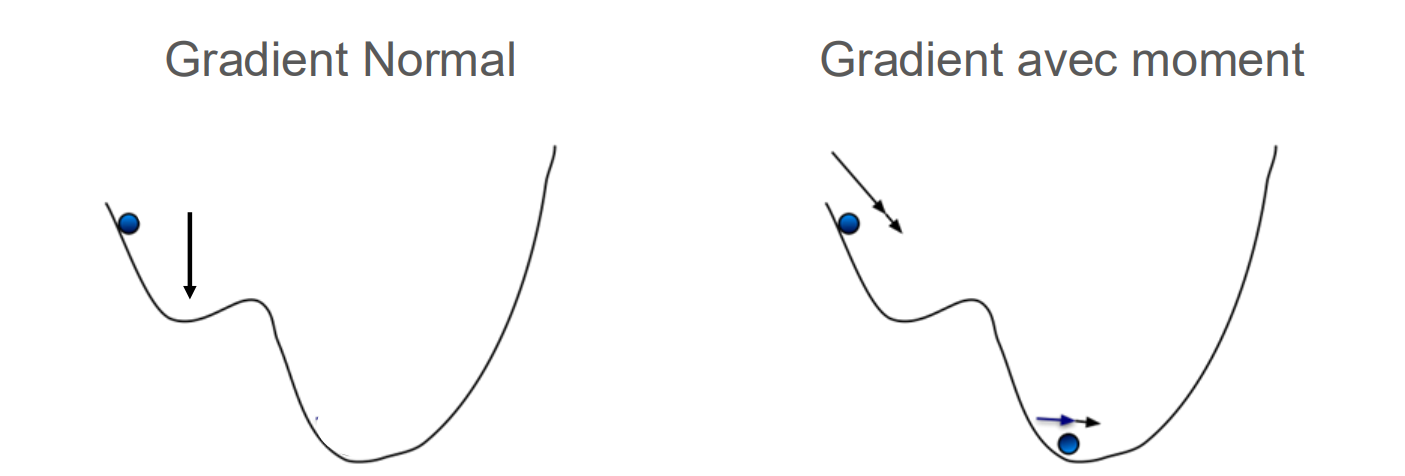
\includegraphics[width=1 \linewidth]{graphics/S3Optimisation/gradient_with_moment.PNG}
    \caption{Gradient avec moment}
    \label{fig:gradient_with_moment}
\end{figure}

La mise à jour des poids en utilisant le gradient avec moment se fait selon la règle suivante :
\[
v_{t+1} = \rho v_t - \eta \nabla L(f(x;\theta_t), y)
\]
\[
\theta^{t+1} = \theta^t + v_{t+1}
\]
where \(\rho\) is the momentum coefficient.

\subsubsection{Nesterov Accelerated Gradient (NAG)}
Une variante du gradient avec moment est le \textbf{moment de Nesterov}, qui prévoit le déplacement avant de calculer le gradient. Cette approche permet d'anticiper le comportement de la fonction de perte et d'améliorer encore davantage la convergence. Elle aide à réduire les oscillations et à améliorer la vitesse d'apprentissage dans des zones planes de l'espace des solutions.

Nesterov Momentum refines the momentum method by first applying a partial update before computing the gradient, allowing for more accurate gradient adjustments.
\[
\tilde{\theta} = \theta + \alpha v,
\]
\[
g = \nabla_\theta L(\tilde{\theta}),
\]
\[
v \leftarrow \alpha v - \eta g,\quad \theta \leftarrow \theta + v.
\]

\subsubsection{ADAGRAD (Adaptive Gradient)}
Adagrad adapts the learning rate for each parameter for each parameter using accumulated squared gradients, making it suitable for convex problems but potentially slowing down over time due to accumulated gradients.
\[
r \leftarrow r + g \odot g,
\]
Here $r$ accumulates past squared gradients element-wise.
\[
\Delta \theta = \frac{\eta}{\sqrt{r} + \epsilon} \odot g,
\]
Here $\epsilon$ is a small constant for numerical stability.
\[
\theta \leftarrow \theta - \Delta \theta.
\]
\subsubsection{RMSPROP}

TODO 

\subsubsection{ADAM (Adaptive Moment Estimation)}
This optimiser combines RMSPROP and momentum, computing adaptive learning rates for each parameter by using both first-order moment estimates (momentum) and second-order moment estimates (variance).

We compute the first moment estimate $m$ (moving average of gradients) and the second moment estimate $v$ (moving average of squared gradients) as 
\[
m \leftarrow \beta_1 m + (1 - \beta_1) g,\quad v \leftarrow \beta_2 v + (1 - \beta_2) g \odot g,
\]
Where $\beta_*$ is is the decay rate.
\[
\hat{m} = \frac{m}{1 - \beta_1^t},\quad \hat{v} = \frac{v}{1 - \beta_2^t},
\]

The bias correction terms $\hat{m}$ and $\hat{v}$ are then used to  adjust for the initialization bias.
\[
\Delta \theta = \frac{\eta}{\sqrt{\hat{v}} + \epsilon} \odot \hat{m},\quad \theta \leftarrow \theta - \Delta \theta.
\]

Adam is widely used due to its robustness and ability to handle sparse gradients.

\subsubsection{ADAMW}
The succesor of ADAM, who is also very popular. This method decouples weight decay from gradient updates, improving generalization.
% TODO add more details

\subsubsection{AMSGRAD}
This optimiser ensures non-increasing second moment estimates to address convergence issues in ADAM.
%TODO add more details

\subsubsection{ADABOUND}
This optimiser dynamically bounds the learning rate to transition smoothly between adaptive methods and SGD.
%TODO add more details

\subsection{Normalization} (NEW)
Normalization accelerates training and stabilizes gradient flow by standardizing activations.

\begin{figure}
    \centering
    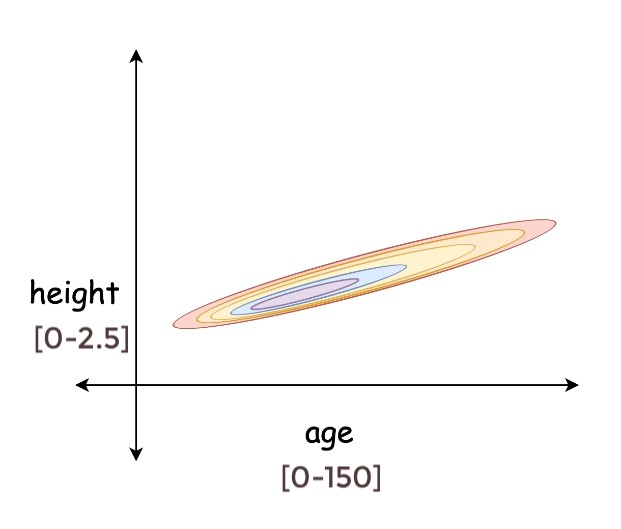
\includegraphics[width=0.4\linewidth]{graphics/S3Optimisation/batchnorm_exp01.jpg}
    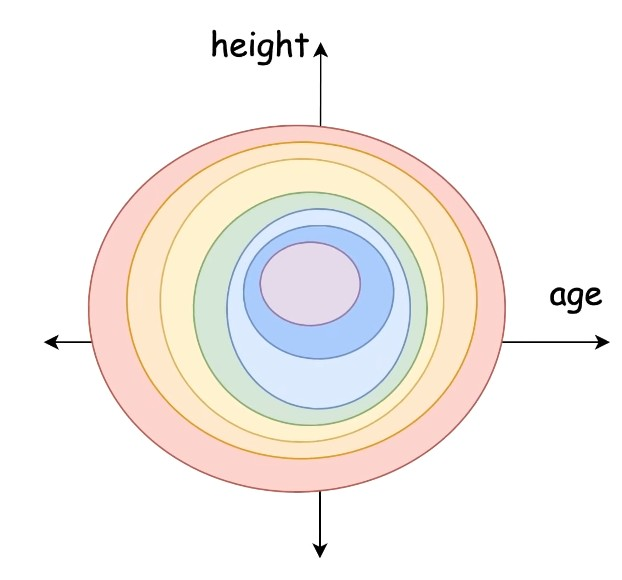
\includegraphics[width=0.4\linewidth]{graphics/S3Optimisation/batchnorm_exp02.jpg}
    \caption{Gradient landscape without and with normalization}
    \label{fig:batchnorm}
\end{figure}

Normalizing inputs (or activations) helps reduce the impact of differing value ranges, smoothing the loss landscape and improving gradient flow.

As we can see in figure \ref{fig:enter-label}, the landscape of normalized data will be much easier to traverse during training. Without it, there are some locations that could be complicated to get out of and some points are much further away than others. In the normalized case, everything is "relatively" close.

This will also make initialization less critical and leads to faster convergence from various starting points.

Once the parameters are normalised, the learned parameters \(\gamma\) and \(\beta\) are applied:
\[
\hat{x}_i = \frac{x_i - \mu}{\sqrt{\sigma^2 + \epsilon}},\quad y_i = \gamma \hat{x}_i + \beta.
\]

In neural networks, we can apply layers of normalisation to the data. In such a layer, for \(D\) features, there are \(2 \times D\) trainable parameters (\(\gamma\) and \(\beta\)).
\textbf{Parameters:}
\[
\text{Total Parameters} = 2 \times D,
\]
accounting for $\gamma$ and $\beta$ per feature (aside from non-trainable running statistics).

\subsubsection{Batch Normalization}
\label{sec:batchnorm}

\textbf{Reference:} Ioffe, Szegedy (ICML 2015)

Batch Normalization (BN) normalizes activations across each channel for all samples in a batch.  
Given batch of examples of size $B$, with channels $C$ and features $F$, we compute:
\[
\mu_c = \frac{1}{B*F} \sum_{B,F} x_{bcf}, 
\quad
\sigma^2_c = \frac{1}{B*F} \sum_{B,F} (x_{bcf} - \mu_c)^2.
\]

\begin{itemize}
    \item Works well in image processing. Typically inserted between linear/convolution layers and the nonlinearity.
    \item Works well for large mini-batch sizes.
\end{itemize}

\subsubsection{Layer Normalization}
\label{sec:layernorm}

\textbf{Reference:} Ba, Kiros, Hinton

Layer Normalization (LN) normalizes across the features (hidden units) within a single layer for each sample. Given batch of examples of size $B$, with channels $C$ and features $F$, we compute:
\[
\mu_b = \frac{1}{C*F} \sum_{C,F} x_{bcf}, 
\quad
\sigma^2_b = \frac{1}{C*F} \sum_{C,F} (x_{bcf} - \mu_b)^2.
\]

\begin{itemize}
    \item Often used in RNNs and Transformers (especially when mini-batches are small or variable in size).
    \item Normalization is independent for each training example.
\end{itemize}

\subsubsection{Instance Normalization}
\label{sec:instancenorm}

Instance Normalization (IN) normalizes across spatial dimensions for each channel and for each sample independently. It is frequently used in style transfer tasks. Given batch of examples of size $B$, with channels $C$ and features $F$, we compute:

\[
\mu_{bc} = \frac{1}{F} \sum_{F} x_{bcf}, 
\quad
\sigma^2_{bc} = \frac{1}{F} \sum_{F} (x_{bcf} - \mu_{bc})^2.
\]

\begin{itemize}
    \item Each sample-channel is normalized independently.
    \item Helps in style transfer by normalizing per-image and per-channel statistics.
\end{itemize}

\subsubsection{RMS Normalization}
\label{sec:rmsnorm}

RMS Normalization (RMSNorm) is similar to LayerNorm but normalizes based on the root mean square of the features rather than the variance:
\[
\mu_{\text{b}}^2 = \frac{1}{C*F} \sum_{C,F} x_{bcf}^2
\quad\text{and}\quad
\hat{x}_{bcf} = \frac{x_{bcf}}{\sqrt{\mu_b^2 + \epsilon}}
\]

\begin{itemize}
    \item Does not subtract a mean; only divides by the root mean square.
    \item Useful in large-scale models due to reduced computational cost compared to LayerNorm.
\end{itemize}

\subsubsection{Group Normalization}
\label{sec:groupnorm}

\textbf{Reference:} Wu and He (2018)

Group Normalization (GN) normalizes by splitting channels into $G$ groups, then normalizing each group’s mean and variance.

\begin{itemize}
    \item Bridges the gap between LayerNorm and InstanceNorm.
    \item Works well when mini-batch sizes are small.
\end{itemize}

\subsubsection{Weight Normalization}
\label{sec:weightnorm}

Weight Normalization (WN) normalizes the weights (rather than activations). It reparameterizes a weight vector $\mathbf{w}$ as
\[
\mathbf{w} = \frac{g}{\|\mathbf{v}\|} \mathbf{v},
\]
where $\mathbf{v}$ is a learned direction and $g$ is a learned scalar. Then the output is:
\[
y = \phi(\mathbf{w} \cdot \mathbf{x} + b).
\]
\begin{itemize}
    \item Decouples the magnitude of the weights from their direction.
    \item Simplifies optimization by controlling the length of the weight vector explicitly.
\end{itemize}

% =============================================================
\clearpage\newpage

\section{Regularization} \label{sec:regularization}
A central problem in machine learning is how to make an algorithm that will perform well not just on the training data, but also on new inputs. Many strategies used in machine learning are explicitly designed to reduce the test error, possibly at the expense of increased training error. These strategies are known collectivelyas regularization. A great many forms of regularization are available to the deep learning practitioner.

\subsection{L2 Regularization}
TODO..
% TODO: Add more details on L2 regularization.

\subsection{L1 Regularization}
TODO..
% TODO: Add more details on L1 regularization.

\subsection{Early Stopping}
This algorithm allows us to stop the training when we see the performance on the validation set reducing.

\subsubsection{Variants}
There exist techniques that are not very used recently but are still worth mentioning such as

\begin{itemize}
\item \textbf{Early Stopping with Retraining:} This technique is made to not waste certain example in the validation set and uses validated examples for a minor performance boost. It's not very popular because it's not the goal to grab this little performance gain and the data base are very big now.
\item \textbf{Early Stopping with Surrogate Loss:} Employs an alternate loss function.
\end{itemize}

\subsection{Dropout Training}
Randomly disables certain connections during training to reduce overfitting.
%TODO add more details 

\subsection{Stochastic Depth}
Randomly drop entire layers during training, particularly effective in ResNets.

\subsection{Transfer Learning}
Train a general model and fine-tune it for specific tasks.

\subsection{Multi-Task Learning}
Build a general model and plug in smaller task-specific modules.
\begin{figure}[ht]
    \centering
    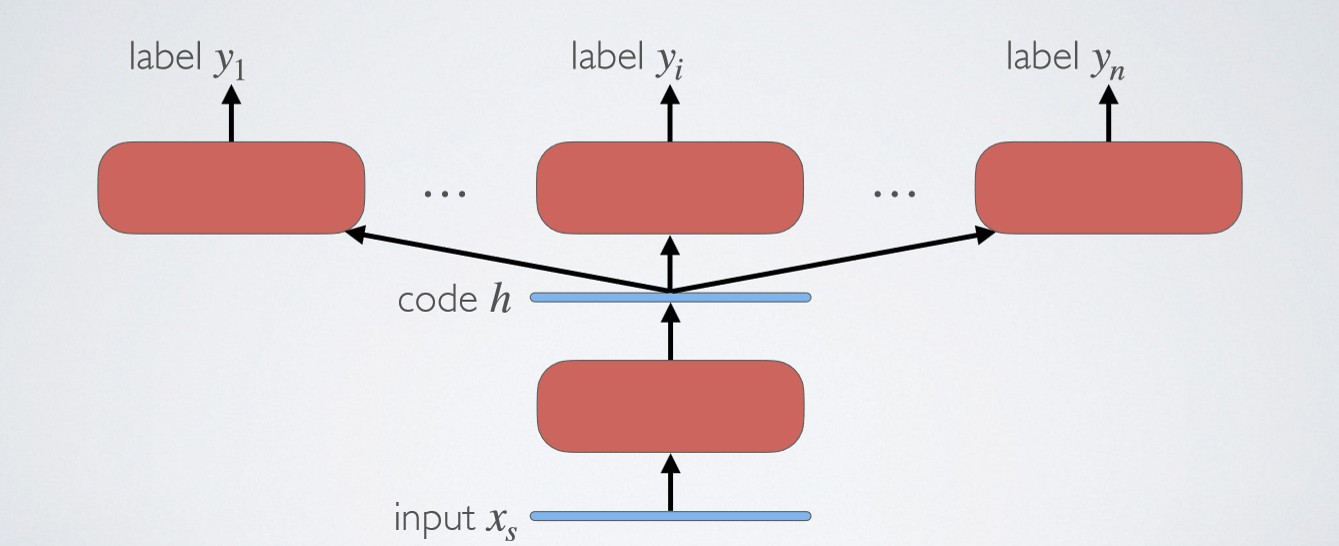
\includegraphics[width=\linewidth]{graphics/S4Regularisation/multitask-learning.jpg}
    \caption{Multi-Task Learning architecture}
    \label{fig:multitask-learning}
\end{figure}

\subsection{Label Smoothing}
Replace hard labels (0 and 1) with smoothed values to improve generalization. This results in a cluster of labels together.
% TODO: Add precise equations.

\begin{figure}
    \centering
    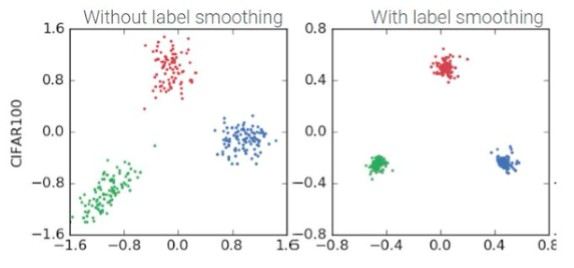
\includegraphics[width=1\linewidth]{graphics/S4Regularisation/label-smoothing.jpg}
    \caption{Source: When does label smoothing help?}
    \label{fig:enter-label}
\end{figure}

\subsection{Data Augmentation}
Increase dataset size by applying transformations (translation, rotation, etc.). This technique had a HUGE impact on the image, audio, video and other tasks with those type of data but NONE to others like text because there is no way found so far to augment text.

\subsubsection{Data Augmentation for Images}
% TODO add visualisation of the techniques

\paragraph{RandAugment} This technique is among the most popular. In general, it applies transformations such as: translation, rotation, scaling, equalization, posterization and solarization, etc...

However, more aggressive augmentation techniques exist..

\paragraph{MixUp} Blends two images and their labels. This technique generally yields low performance.

\paragraph{Random Erasing / Cutout} Removes a random portion of the image.

\paragraph{CutMix} Combines regions from different images with proportional labels.

% =============================================================
\clearpage\newpage

\section{Convolutional Neural Networks (CNNs)} \label{sec:cnn}
% TODO adding something from this might be interesting : https://guandi1995.github.io/Pooling-Layers/#:~:text=In%20summary%2C%20since%20there%20are,1%20%E2%8C%8B%20%C3%97%20n%20c%20.

A Convolutional Neural Network (CNN) is a type of neural network designed specifically for pattern recognition in image or audio data (mimicking the way the visual cortex processes visual information). CNNs leverage convolution operations to extract hierarchical features from images, efficiently handling high-dimensional data while exploiting spatial structures, such as the relationship between nearby pixels. This architecture builds invariance to transformations like translation, making it highly effective for image-related tasks. A typical CNN consists of alternating convolutional and pooling layers, followed by fully connected layers.

\subsection{Key Features}
\paragraph{Local Connectivity} Each neuron connects only to a local region of the input, called the \textit{receptive field}. This allows CNNs to focus on localized patterns (e.g., edges, textures), reducing the number of parameters compared to fully connected networks (FFNs).

\paragraph{Parameter Sharing} The same set of weights (kernel) is used across different spatial locations of the input, significantly reducing computational complexity.
\paragraph{Pooling (Dimensionality Reduction)} Reduces the number of hidden units in the model and helps achieve translational invariance, improving generalization.

For an image \(x\), a kernel \(k\), and output \(y\):
\[
(y * k)_{i,j} = \sum_{p,q} x_{i+p,j+q} \cdot k_{r-p, r-q}.
\]

\subsection{Convolution Layer}
For an input of size \(N \times N \times D_{in}\), kernel of size \(K \times K\), stride \(S\), padding \(P\), and \(D_{out}\) filters:
\[
N_{out} = \left\lfloor \frac{N - K + 2P}{S} \right\rfloor + 1,
\]
with total parameters:
\[
\text{Total Parameters} = D_{out} \times \left( K \times K \times D_{in} + \text{(bias term)} \right).
\]

\subsection{Pooling Layer}
For input of size \(N \times N \times D\), pooling window \(F \times F\), and stride \(S\):
\[
N_{out} = \left\lfloor \frac{N - F}{S} \right\rfloor + 1,
\]
with zero trainable parameters. There are two main types of pooling

\begin{itemize}
    \item \textbf{Max Pooling:}
    \[
    y_{i,j} = \max_{(p,q) \in R} x_{i+p, j+q}.
    \]
    \item \textbf{Average Pooling:}
    \[
    y_{i,j} = \frac{1}{|R|} \sum_{(p,q) \in R} x_{i+p, j+q}.
    \]
\end{itemize}

\subsection{Stride and Padding}
\paragraph{Stride} Controls the step size of the convolutional filter when moving across the input.

\paragraph{Padding} Adds extra pixels around the input to control output size. Special cases include:
\begin{itemize}
    \item \textbf{Valid Convolution} ($P=0$): no padding, spatial dimensions shrink.
    \item \textbf{Same Convolution} ($P=\lfloor d\,(K-1)/2\rfloor$): half (or “same”) padding, preserves spatial dimensions.
    \item \textbf{Full Convolution} ($P=K-1$): full padding, maximizes overlap so the output is larger than the input.
\end{itemize}

\begin{figure}[ht]
    \centering
    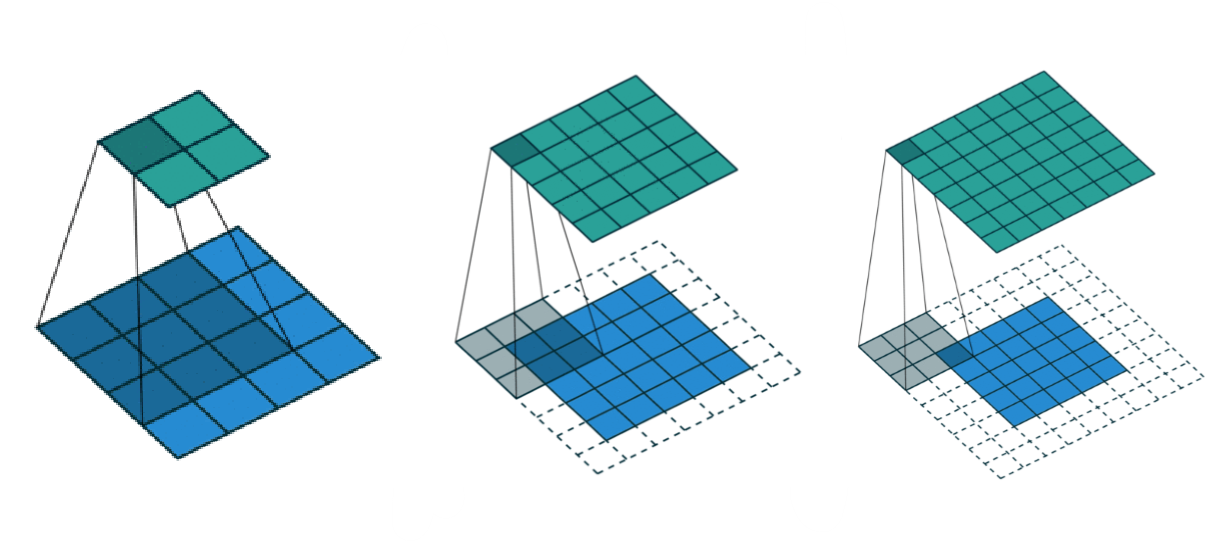
\includegraphics[width=0.7\linewidth]{graphics/S5CNN/padding_cnn.png}
    \caption{Special padding cases for a 2D convolution: to the left valid convolution (no padding), in the middle same convolution (input and output dimensions are the equal), and to the right full convolution (maximum padding).}
    \label{fig:padding-cnn}
\end{figure}

\subsection{Receptive Field}

The \emph{receptive field} of a neuron in a convolutional neural network (CNN) is the region of the input that influences that neuron's output. As you progress deeper into the network, the receptive field generally increases, allowing the network to capture larger context. Understanding the receptive field is essential because it helps you design architectures that capture enough context from the input.

\begin{figure}[ht]
    \centering
    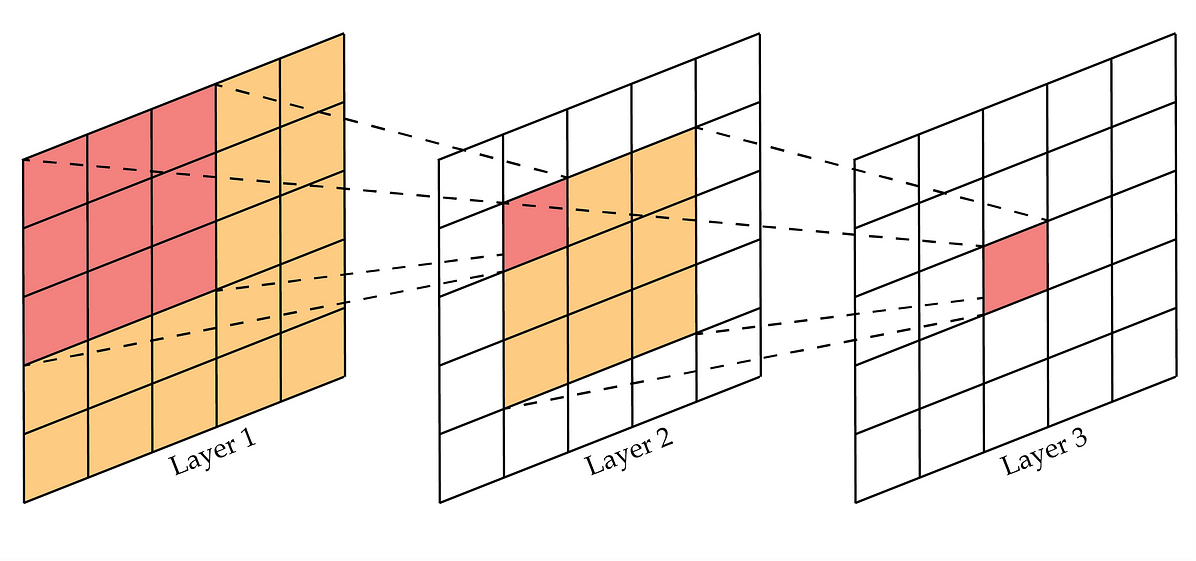
\includegraphics[width=0.7\linewidth]{graphics/S5CNN/receptive_field.png}
    \caption{Receptive field expansion in a deep CNN using consecutive $3\times3$ kernels. Source: Reza Kalantar, “Receptive Fields in Deep Convolutional Networks,” Medium (2019).}
    \label{fig:receptive-field}
\end{figure}

In simpler terms, it is the size of the patch in the input image that contributes to a particular feature in a deeper layer. For layer \(i\) with kernel \(k_i\) and stride \(s_i\), the receptive field can be computed recursively
\[
r_i = r_{i-1} + (k_i - 1) \times S_{i-1},
\]
where \(S_{i-1} = \prod_{j=1}^{i-1} s_j\) is the effective stride. Also, for the first layer applied directly on the input, the receptive field is simply
\[
r_1 = k_1.
\]

\subsection{Backpropagation (TODO)}

\subsection{Dilated Convolutions}
Dilated convolutions “inflate” the kernel by inserting spaces between its elements, thereby expanding the network’s receptive field without extra parameters or computation.

They are especially useful when nearby inputs are highly redundant, and have been employed in sequence–modeling architectures such as WaveNet (see \ref{wavenet}) and ByteNet (see \ref{bytenet}).

\paragraph{Dilation factor}
A hyperparameter $d\ge1$ that inserts $d-1$ “holes” between successive kernel elements.

\paragraph{Effective kernel size}
Denote the original kernel size by $k$.  A dilated kernel of size $k$ and rate $d$ has an effective size
\[
\hat k
= k + (k-1)\,(d-1)
= d\,(k-1) + 1.
\]
Larger $\hat k$ directly increases the receptive field.

\begin{figure}[ht]
    \centering
    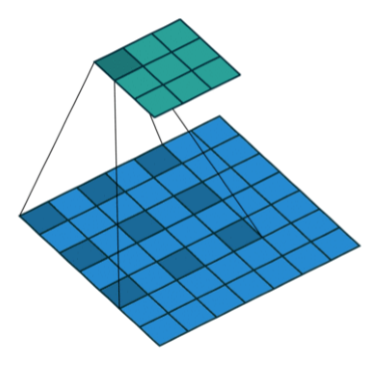
\includegraphics[width=0.3\linewidth]{graphics/S5CNN/dilated_conv.png}
    \caption{Dilated convolution with $i=7$, kernel $k=3$, dilation rate $d=2$, stride $s=1$, and padding $p=0$, yielding an effective kernel size $\hat k = 5$.}
    \label{fig:dilated-conv}
\end{figure}

\subsection{Transpose Convolutions}
Transpose convolutions (also called “deconvolutions”) is the natural “inverse” of the convolution operation. It perform learnable upsampling by reversing the forward pass of a convolution. They are widely used in decoder architectures for image generation or semantic segmentation.  

\subsection{Separable Convolutions}
Separable convolutions factorize a standard convolution into two smaller operations—depthwise and pointwise—to reduce parameters and computation.

\paragraph{Depthwise convolution}
Applies a $k\times k$ filter to each input channel separately:
\[
\text{FLOPs}_{\mathrm{dw}}
= H_{\mathrm{in}}W_{\mathrm{in}} \,\times\,k^2\,C_{\mathrm{in}}.
\]

\paragraph{Pointwise convolution}
Follows with a $1\times1$ convolution to linearly combine the $C_{\mathrm{in}}$ channels into $C_{\mathrm{out}}$:
\[
\text{FLOPs}_{\mathrm{pw}}
= H_{\mathrm{in}}W_{\mathrm{in}} \,\times\,C_{\mathrm{in}}\,C_{\mathrm{out}}.
\]

\paragraph{Parameter reduction}
Compared to a standard $k\times k$ convolution ($k^2C_{\mathrm{in}}C_{\mathrm{out}}$ parameters), depthwise separable uses
\[
k^2C_{\mathrm{in}} \;+\; C_{\mathrm{in}}C_{\mathrm{out}},
\]
often yielding a 5–10× reduction in computation for typical network widths.


\subsection{Architectural Taxonomy}

\subsubsection{ResNet (Residual Networks)}
Deep networks suffer from the \textit{vanishing gradient problem}, where gradients become too small to update weights effectively. ResNet introduces skip connections, allowing layers to learn residual mappings:
\[
F(x) = H(x) - x,
\]
where $H(x)$ is the desired underlying mapping. This enables stable training of very deep models (e.g.\ ResNet‑50, ResNet‑152).

\begin{figure}[ht]
    \centering
    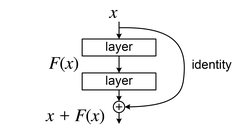
\includegraphics[width=0.35\linewidth]{graphics/S5CNN/ResBlock.png}
    \caption{Structure of a ResNet residual block. The input $x$ is added to the output of the residual function $F(x)$ via a skip connection.}
    \label{fig:resnet-resblock}
\end{figure}

There are two types of residual blocks:

\paragraph{Basic Block}
Used in shallower ResNets (e.g.\ ResNet‑18/34). It consists of two $3\times3$ convolutions, each followed by BatchNorm and ReLU, plus an identity shortcut.

\paragraph{Bottleneck Block}
Used in deeper variants (e.g.\ ResNet‑50/101/152). It stacks a $1\times1$ projection (reduce channels), a $3\times3$ convolution, and a $1\times1$ expansion, all with BatchNorm and ReLU, plus a shortcut.

\begin{figure}[ht]
    \centering
    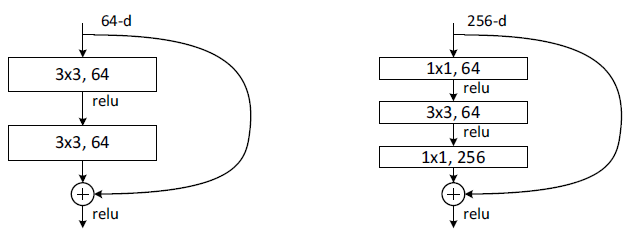
\includegraphics[width=0.65\linewidth]{graphics/S5CNN/res_blocks_type.png}
    \caption{Comparison of ResNet block types. 
    \textbf{Left}: basic block (two 3×3 convolutions).}
    \label{fig:resnet-block-types}
    \textbf{Right}: bottleneck block (1×1, 3×3, 1×1 convolutions);
\end{figure}

\subsubsection{SENet (Squeeze-and-Excitation Networks)}
SENet introduces a lightweight channel‑wise attention mechanism:
\begin{enumerate}
    \item \textbf{Squeeze:} Global average pooling produces a per‑channel descriptor.
    \item \textbf{Excitation:} Two small FC layers (with bottleneck) learn channel weights via a sigmoid.
    \item \textbf{Recalibration:} These weights rescale the original feature maps.
\end{enumerate}
This adaptively emphasises informative channels with minimal cost.

\subsubsection{WaveNet}\label{wavenet}
A generative model for raw audio signals. WaveNet stacks causal, dilated $1$D convolutions with exponentially increasing dilation rates, interleaved with gated activations and residual/skip connections. It models long-range dependencies without recurrence and outputs sample‑by‑sample distributions via a softmax over quantised amplitudes.

\subsubsection{ByteNet}\label{bytenet}
A fully convolutional sequence‑to‑sequence model for text. ByteNet uses two stacks of dilated convolutions: an encoder to build representations of the source sequence, and an autoregressive decoder that conditions on previous outputs. Residual connections and causal masking ensure efficient, parallelisable training and linear inference time.

\subsubsection{EfficientNet}
EfficientNet achieves state‑of‑the‑art accuracy through \emph{compound scaling}: jointly scaling network depth, width, and input resolution by a set of coefficients found via small‑grid search. It builds on MobileNetV2’s MBConv blocks (inverted residual + squeeze‑and‑excitation) to maximise performance per FLOP.

\subsubsection{ConvNeXt}
ConvNeXt modernises the classic CNN by incorporating design elements inspired by Vision Transformers:  
\begin{itemize}
  \item Replace $3\times3$ convs with large‑kernel depth‑wise convs (e.g.\ $7\times7$).
  \item Use LayerNorm in “channels-last” format.
  \item Swap ReLU+BN for GELU+LayerNorm.
  \item Maintain a simple macro‑architecture (ResNet‑style stages and downsampling).
\end{itemize}
These changes yield competitive accuracy on ImageNet with similar compute to large transformer models.

% =============================================================
\clearpage\newpage

\section{Recurrent Neural Networks (RNN)}

Recurrent Neural Networks (RNNs) are a class of neural networks specifically designed to handle sequential data, making them ideal for tasks such as language modeling, speech recognition, and machine translation. Their strength lies in their ability to maintain a persistent hidden state across time steps, allowing them to capture temporal dependencies within the data. Despite their early success, RNNs have been largely overshadowed by transformers (see \ref{sec:transformers}), which have proven to be more efficient and effective in handling long-range dependencies and parallel computation.

\begin{figure}[ht]
    \centering
    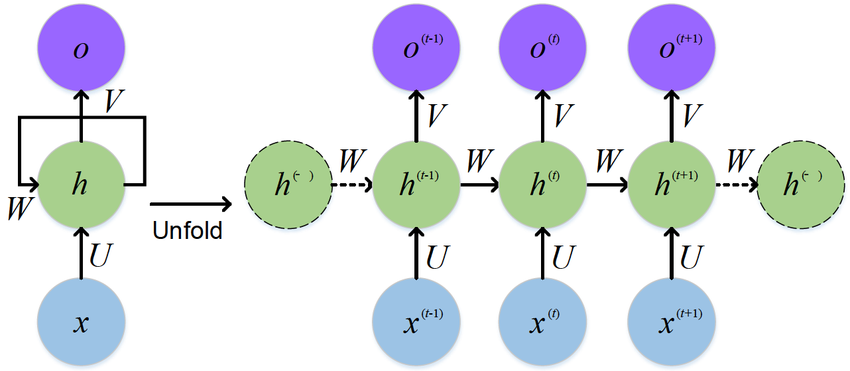
\includegraphics[width=0.6\linewidth]{graphics/S6RNN/rnn-unrolledrnn.png}
    \caption{Unrolled recurrent neural network over multiple time steps, depicting hidden state propagation and input–output dependencies in an audio‑visual speech recognition model. Source: Feng et al. (2017).}
    \label{fig:unrolled-rnn}
\end{figure}

RNNs process sequential data by maintaining a hidden state that evolves over time. At each time step \(t\), the hidden state \(h_t\) is updated based on the previous hidden state \(h_{t-1}\) and the current input \(x_t\):
\[
h_t = f(h_{t-1}, x_t)
\]

The output \(y_t\) is then computed from the hidden state:
\[
y_t = \text{softmax}(W h_t + b)
\]
where \(W\) is the weight matrix and \(b\) is the bias term. 

This recurrence allows the model to retain information from earlier time steps, making it suitable for tasks where context plays a crucial role in understanding the sequence.

\subsection{Backpropagation Through Time (BPTT)}
Backpropagation Through Time (BPTT) is the method used to train RNNs by applying backpropagation to the unrolled network over time. The network is "unrolled" for the number of time steps corresponding to the input sequence. The gradients are computed and propagated backward through the unrolled graph.

\subsubsection{Truncated BPTT}
Truncated BPTT is a practical modification where, instead of unrolling the network for the entire sequence, the network is unrolled for a fixed number of time steps, \(k\). This approximation helps reduce computational complexity and memory usage, especially when dealing with long sequences. Truncated BPTT also helps mitigate issues like vanishing gradients by limiting the range over which gradients are propagated.

\subsection{Exploding Gradient Problem}
The exploding gradient problem occurs when the gradients grow exponentially during backpropagation. This is typically caused by repeated multiplication of gradients by values greater than 1. In such cases, the gradients can become very large, causing the model's weights to update in large, unstable steps. This can lead to numerical overflow or an inability to converge during training.

Mathematically, the exploding gradient problem is the opposite of the vanishing gradient problem. If the term \(\frac{\partial h_{t+1}}{\partial h_t}\) is greater than 1, the gradients will increase exponentially as they are propagated back through the network:

\[
\frac{\partial L}{\partial h_t} = \frac{\partial L}{\partial h_{t+1}} \cdot \frac{\partial h_{t+1}}{\partial h_t}
\]

This problem leads to instability in the training process, where the weights may fluctuate wildly, preventing the model from finding an optimal solution.

\subsubsection{Gradient Clipping}
Gradient clipping is a solution to the exploding gradient problem. It involves rescaling the gradients if their norm exceeds a specified threshold, preventing them from growing too large and causing instability in the learning process:

\[
\mathbf{g} = \frac{\mathbf{g}}{\|\mathbf{g}\|} \cdot \text{threshold}, \quad \text{if} \quad \|\mathbf{g}\| > \text{threshold}
\]

This technique ensures that the gradients do not cause the model's weights to make large, unstable updates.

\subsection{Vanishing Gradient Problem}
The vanishing gradient problem occurs when the gradients shrink exponentially as they are propagated back through time. This happens because the gradients are repeatedly multiplied by values smaller than 1 (e.g., activation functions like \(\tanh\) or sigmoid squash their inputs to a small range). Over many time steps, this multiplication causes the gradients to decay towards zero, making it difficult for the model to learn long-range dependencies.

Mathematically, for an RNN, the gradients are propagated back through the network as:

\[
\frac{\partial L}{\partial h_t} = \frac{\partial L}{\partial h_{t+1}} \cdot \frac{\partial h_{t+1}}{\partial h_t}
\]

If the term \(\frac{\partial h_{t+1}}{\partial h_t}\) is less than 1 for each time step, the gradient will diminish as it is propagated back through many layers, leading to a vanishing gradient.

This problem makes it very difficult for RNNs to capture long-term dependencies. As a result, models struggle to remember important information from earlier time steps in a sequence.

\subsubsection{Orthogonal Initialization}
Orthogonal initialization helps mitigate the vanishing gradient problem. By initializing the weight matrices \(U\) as orthogonal matrices, we ensure that the gradients do not shrink exponentially as they propagate through the network. This helps maintain stable learning over many time steps:

\[
U^\top U = U U^\top = I
\]

where \(I\) is the identity matrix. This ensures that the weight matrix does not distort the signal as it is passed through the network, helping to preserve the magnitude of gradients during training.

\subsection{Architectural Taxonomy}
RNNs have several important variants that enhance their ability to model complex temporal dependencies. Below, we discuss some of the most popular architectures used in practice.

\begin{figure}[ht]
    \centering
    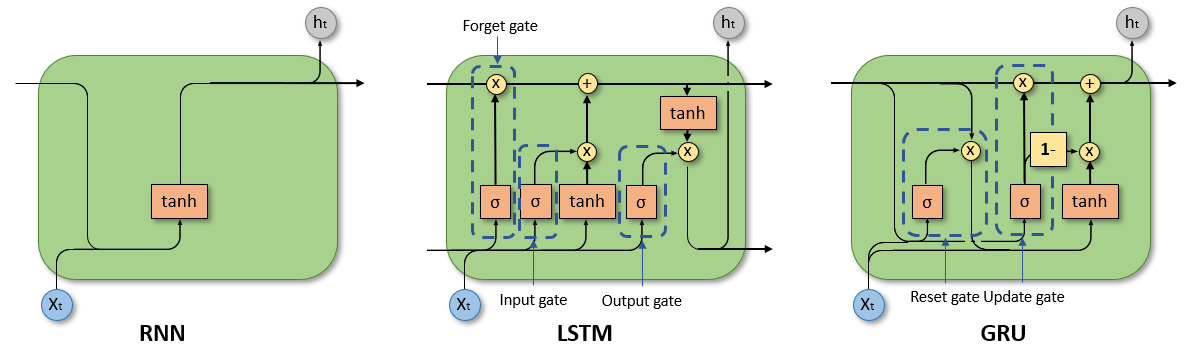
\includegraphics[width=0.9\linewidth]{graphics/S6RNN/rnn_architectures.png}
    \caption{Comparison of standard RNN, LSTM, and GRU architectures, illustrating their recurrent connections and gating mechanisms. Source: Suvankar Maity, LinkedIn.}
    \label{fig:rnn-architectures}
\end{figure}

\subsubsection{LSTM (Long Short-Term Memory)}
LSTM is a type of RNN designed to avoid the vanishing gradient problem by introducing memory cells. These cells maintain information over time and use gates to control the flow of data. The key components of an LSTM are the input gate, forget gate, and output gate:
\[
i_t = \sigma(W_i x_t + U_i h_{t-1}), \quad f_t = \sigma(W_f x_t + U_f h_{t-1}), \quad o_t = \sigma(W_o x_t + U_o h_{t-1})
\]
\[
c_t = f_t \cdot c_{t-1} + i_t \cdot \tilde{c}_t, \quad h_t = o_t \cdot \tanh(c_t)
\]
where \(c_t\) is the cell state, \(i_t\) is the input gate, \(f_t\) is the forget gate, and \(o_t\) is the output gate.

\begin{figure}[ht]
    \centering
    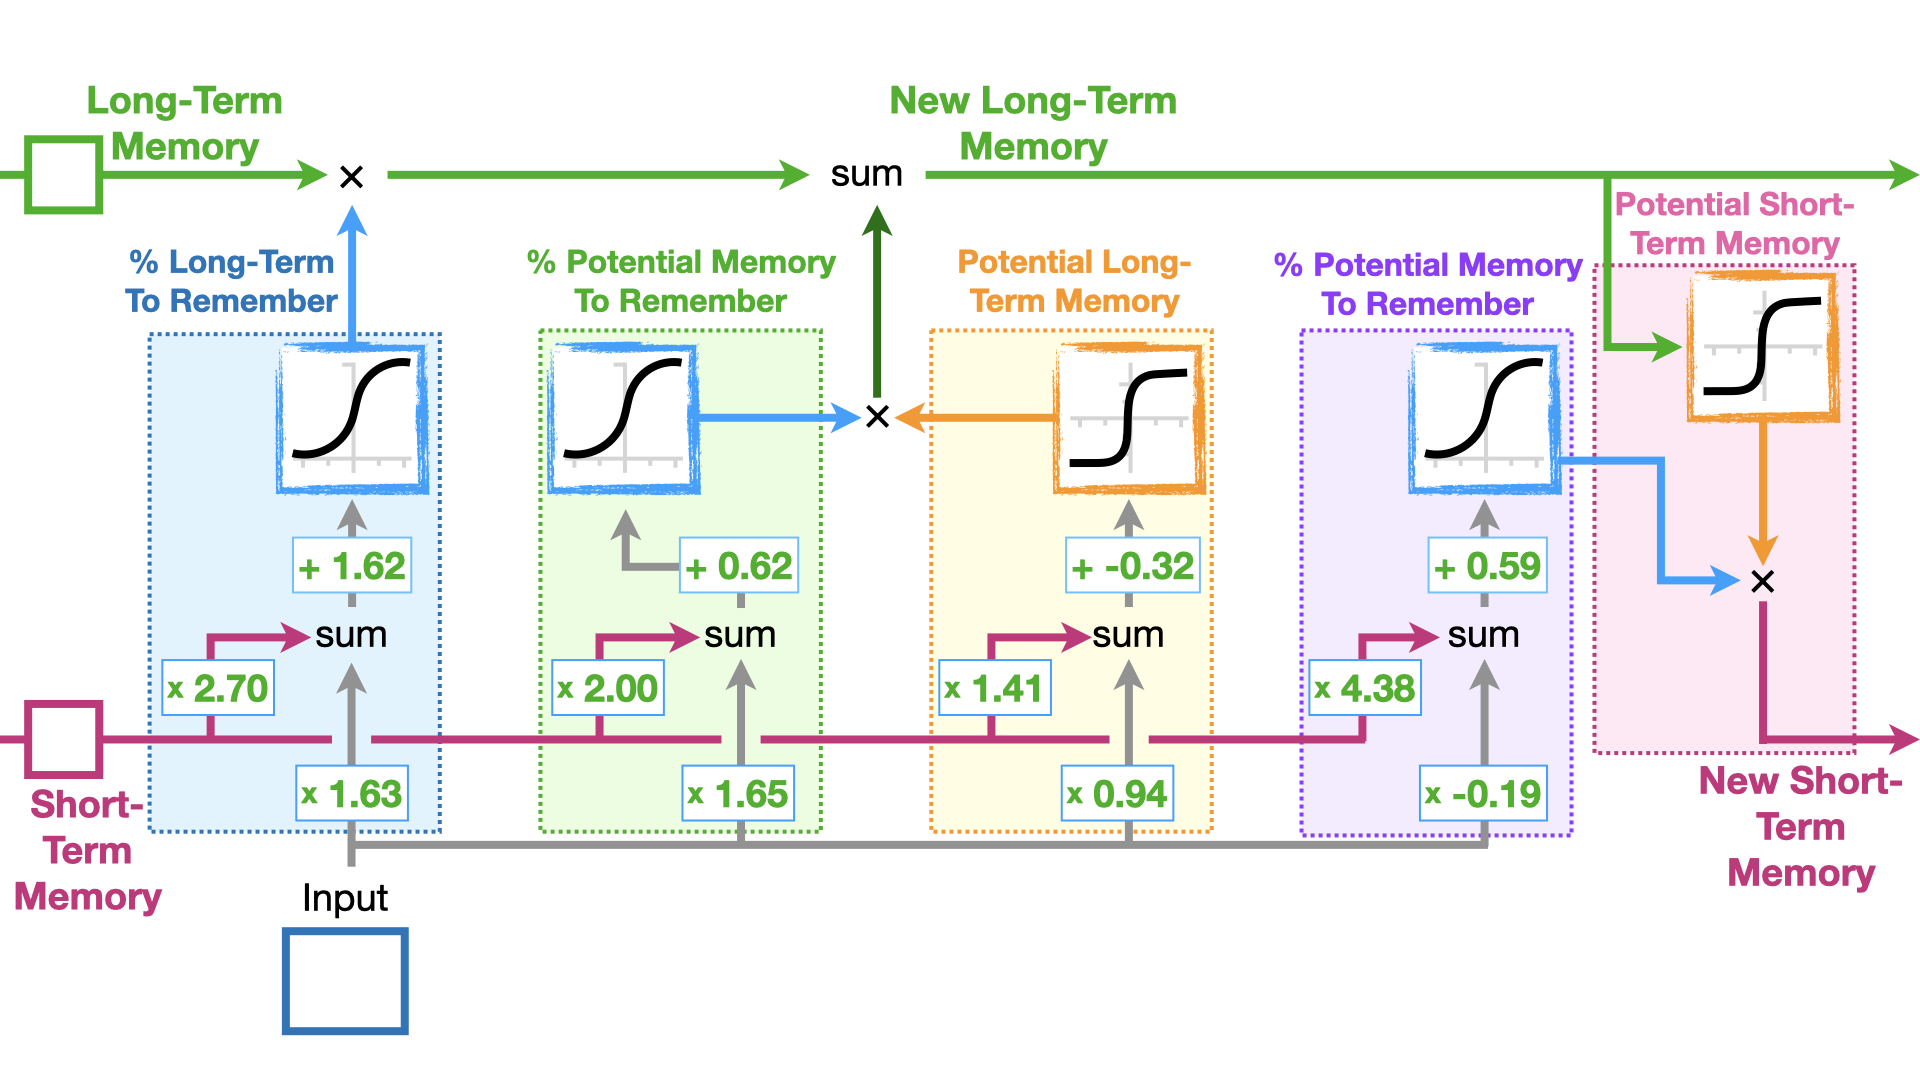
\includegraphics[width=0.9\linewidth]{graphics/S6RNN/lstm_maths.png}
    \caption{Structure of a Long Short‑Term Memory (LSTM) unit showing the input, forget, and output gates along with the cell state update. Source: Josh Starmer, Lightning AI.}
    \label{fig:lstm-unit}
\end{figure}

For more in-depth learning about LSTMs, the following resources are highly recommended:
\begin{itemize}
    \item \href{https://colah.github.io/posts/2015-08-Understanding-LSTMs/}{Colah's Blog - Understanding LSTMs}
    \item \href{https://www.youtube.com/watch?v=YCzL96nL7j0}{Josh Starmer's YouTube Video Explaining LSTMs}
\end{itemize}

\subsubsection{GRU (Gated Recurrent Unit)}
GRU is a variant of LSTM with fewer gates. It uses two gates: the update gate \(z_t\) and the reset gate \(r_t\). These gates control the amount of information to be retained or discarded at each time step:
\[
z_t = \sigma(W_z x_t + U_z h_{t-1}), \quad r_t = \sigma(W_r x_t + U_r h_{t-1})
\]
\[
h_t = (1 - z_t) \cdot h_{t-1} + z_t \cdot \tilde{h}_t
\]
GRUs are simpler than LSTMs but perform similarly in many tasks.



\subsubsection{Seq2Seq (Sequence to Sequence)}
Seq2Seq models use RNNs to map one sequence to another, making them ideal for tasks like machine translation. The architecture consists of an encoder RNN, which processes the input sequence, and a decoder RNN, which generates the output sequence:
\[
h_t = f(h_{t-1}, x_t), \quad y_t = \text{Decoder}(h_t)
\]
Seq2Seq models can use LSTMs or GRUs for both the encoder and decoder.

\subsubsection{Bidirectional RNN}
Bidirectional RNNs (BiRNNs) process each sequence in two directions—forward and backward—allowing the model to incorporate both past and future context when making predictions. At each time step \(t\), the forward and backward hidden states are computed as
\[
h^{(f)}_t = \tanh\bigl(W^{(f)} x_t + U^{(f)} h^{(f)}_{t-1}\bigr), 
\qquad
h^{(b)}_t = \tanh\bigl(W^{(b)} x_t + U^{(b)} h^{(b)}_{t+1}\bigr),
\]
and the output is formed by combining these two states:
\[
y_t = V^{(f)} h^{(f)}_t \;+\; V^{(b)} h^{(b)}_t.
\]
Here, 
\(W^{(f)}, W^{(b)}, U^{(f)}, U^{(b)}, V^{(f)}, V^{(b)}\in\mathbb{R}^{d\times d}\),
and \(x_t,h^{(f)}_t,h^{(b)}_t\in\mathbb{R}^d\) for all \(t\in[1,T]\).

The forward RNN (\(f\)) captures information from the past, while the backward RNN (\(b\)) captures information from the future; their concatenation (or sum) enriches the representation used for each prediction.

\begin{figure}[ht]
\centering
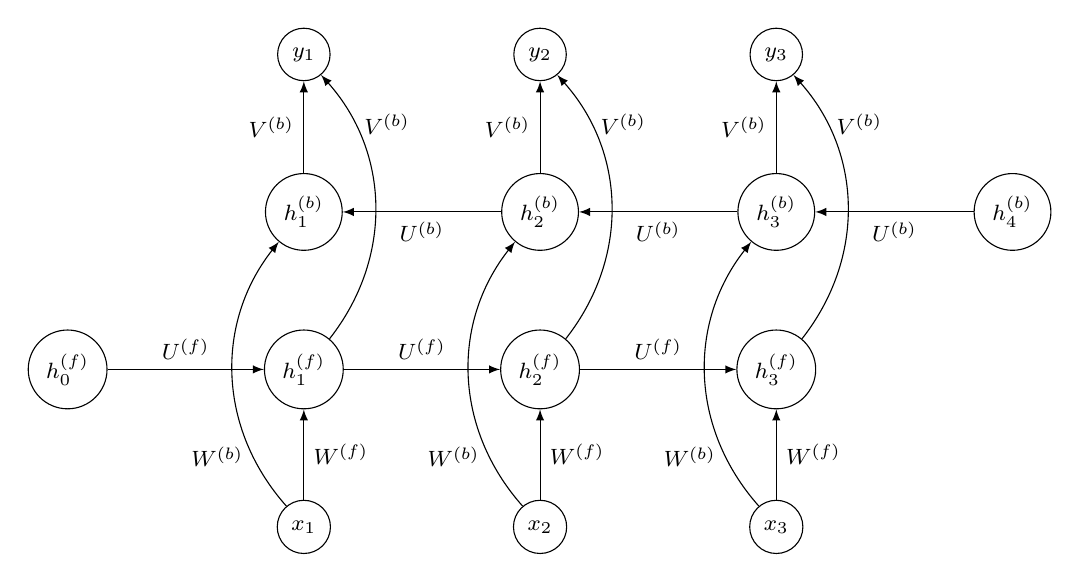
\begin{tikzpicture}[%
    >=latex,              % arrow style
    node distance=2cm,    % base distance between nodes
    on grid,
    every node/.style={font=\footnotesize},
    inputnode/.style={draw, circle, minimum size=6mm},
    hiddennode/.style={draw, circle, minimum size=6mm},
    outputnode/.style={draw, circle, minimum size=6mm},
    ]

%==================================================
% Coordinates
%==================================================

\coordinate (C0) at (-3,0);
\coordinate (C1) at (0,0);
\coordinate (C2) at (3,0);
\coordinate (C3) at (6,0);
\coordinate (C4) at (9,0);

%==================================================
% Input nodes
%==================================================
\node[inputnode] (x1) at (C1)        {\(x_1\)};
\node[inputnode] (x2) at (C2)        {\(x_2\)};
\node[inputnode] (x3) at (C3)        {\(x_3\)};

%==================================================
% Output nodes
%==================================================

\node[outputnode] (y1) at ($(C1)+(0,6)$) {\(y_1\)};
\node[outputnode] (y2) at ($(C2)+(0,6)$) {\(y_2\)};
\node[outputnode] (y3) at ($(C3)+(0,6)$) {\(y_3\)};

%==================================================
% Hidden nodes
%==================================================
% Forward RNN
\node[hiddennode] (hf0) at ($(C0)+(0,2)$) {\(h_0^{(f)}\)};
\node[hiddennode] (hf1) at ($(C1)+(0,2)$) {\(h_1^{(f)}\)};
\node[hiddennode] (hf2) at ($(C2)+(0,2)$) {\(h_2^{(f)}\)};
\node[hiddennode] (hf3) at ($(C3)+(0,2)$) {\(h_3^{(f)}\)};

% Backward RNN
\node[hiddennode] (hb1) at ($(C1)+(0,4)$) {\(h_1^{(b)}\)};
\node[hiddennode] (hb2) at ($(C2)+(0,4)$) {\(h_2^{(b)}\)};
\node[hiddennode] (hb3) at ($(C3)+(0,4)$) {\(h_3^{(b)}\)};
\node[hiddennode] (hb4) at ($(C4)+(0,4)$) {\(h_4^{(b)}\)};

%==================================================
% Arrows
%==================================================
% Forward RNN
\draw[->] (x1) -- node[right]{\(W^{(f)}\)} (hf1);
\draw[->] (x2) -- node[right]{\(W^{(f)}\)} (hf2);
\draw[->] (x3) -- node[right]{\(W^{(f)}\)} (hf3);

\draw[->, bend right=40] (hf1) to node[pos=0.8, right] {\(V^{(b)}\)} (y1);
\draw[->, bend right=40] (hf2) to node[pos=0.8, right] {\(V^{(b)}\)} (y2);
\draw[->, bend right=40] (hf3) to node[pos=0.8, right] {\(V^{(b)}\)} (y3);

\draw[->] (hf0) -- node[above]{\(U^{(f)}\)} (hf1);
\draw[->] (hf1) -- node[above]{\(U^{(f)}\)} (hf2);
\draw[->] (hf2) -- node[above]{\(U^{(f)}\)} (hf3);

% Backward RNN
\draw[->, bend left=40] (x1) to node[pos=0.2, left] {\(W^{(b)}\)} (hb1);
\draw[->, bend left=40] (x2) to node[pos=0.2, left] {\(W^{(b)}\)} (hb2);
\draw[->, bend left=40] (x3) to node[pos=0.2, left] {\(W^{(b)}\)} (hb3);

\draw[->] (hb3) -- node[left]{\(V^{(b)}\)} (y3);
\draw[->] (hb2) -- node[left]{\(V^{(b)}\)} (y2);
\draw[->] (hb1) -- node[left]{\(V^{(b)}\)} (y1);

\draw[->] (hb4) -- node[below]{\(U^{(b)}\)} (hb3);
\draw[->] (hb3) -- node[below]{\(U^{(b)}\)} (hb2);
\draw[->] (hb2) -- node[below]{\(U^{(b)}\)} (hb1);

%==================================================
\end{tikzpicture}
\caption{Unrolled bidirectional RNN over three time steps, showing the forward and backward hidden states (\(h^{(f)}\) and \(h^{(b)}\)), their recurrent connections (\(U^{(\cdot)}\)), input connections (\(W^{(\cdot)}\)), and output projections (\(V^{(\cdot)}\)).}
\label{fig:bidirectional-rnn}
\end{figure}


\subsubsection{State Space Models (SSM)}
State Space Models (SSMs) generalize RNNs by representing the system dynamics as continuous state transitions. SSMs efficiently model long-term dependencies by leveraging structured latent states.

\paragraph{HIPPO (Harmonic Infinite Order Polynomial ODE)}
The HIPPO framework formulates SSMs using polynomial Ordinary Differential Equations (ODEs). It introduces a harmonic structure that improves the modeling of long-range dependencies by providing a smooth transition between states across time.

\subsubsection{S4 (Structured State Space Model)}
The S4 model builds on SSMs by leveraging structured state spaces for efficient sequence modeling. By employing matrix decompositions, S4 can handle long sequences more effectively than traditional RNNs, providing better scalability and computational efficiency.

\subsubsection{MAMBA (Masked Multi-Head Attention RNN)}
MAMBA is a hybrid architecture that combines the benefits of attention mechanisms with RNNs. It uses masked attention heads to focus on relevant parts of the input sequence while processing it, improving performance on tasks like sequence labeling and machine translation.




% =============================================================
\clearpage\newpage

\section{Transformers} \label{sec:transformers}
Transformers are effective for language modeling due to their ability to process data in parallel and capture long-range dependencies through attention.

Here are some key points when fine-tuning this type of model:
\begin{itemize}
    \item The dimension of attention keys is critical.
    \item Larger models generally achieve better performance.
    \item Dropout is beneficial.
    \item Positional encodings (sinusoidal or learned) produce similar results.
\end{itemize}

\subsection{Attention Mechanism}
\textit{TODO: This concept needs a dedicated sub section to clearly explain it}
% TODO: Describe the self-attention mechanism in more details

\subsection{Temperature in Transformers}
Temperature is a scaling factor used to control the probability distribution in the self-attention mechanism and during text generation. It modulates the model’s "confidence" in its predictions by adjusting the sharpness of the distributions. Temperature scales the softmax in both self-attention and text generation:

\paragraph{Self-Attention}
\[
e_{ij} = \frac{Q_i \cdot K_j^T}{T\sqrt{d_k}},
\]
where \(T\) adjusts the sharpness.

\paragraph{Text Generation}
\[
P(y) = \operatorname{softmax}\left(\frac{z}{T}\right).
\]

In other words, the parameter \( T \) influences the attention distribution:
\begin{itemize}
    \item \textbf{Low Temperature (\( T < 1 \))}: Results in a sharper distribution, concentrating more strongly on a few tokens with high scores.
    \item \textbf{High Temperature (\( T > 1 \))}: Produces a more diffuse distribution, allowing broader but less pronounced attention.
\end{itemize}


\subsection{Architectural Taxonomy}
\begin{figure}[ht]
    \centering
    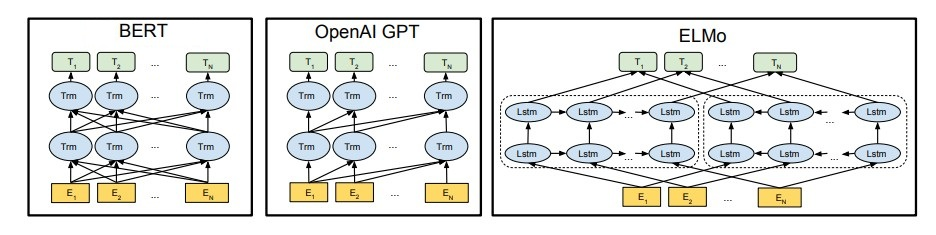
\includegraphics[width=\linewidth]{graphics/S7Transformers/transformers_architectures.jpg}
    \caption{Architecture des Transformers. Source : \textit{BERT: Pre-training of Deep Bidirectional Transformers for Language Understanding} (Devlin et al.)}
    \label{fig:transformers_architecture}
\end{figure}

\subsubsection{GPT (Generative Pre-trained Transformer)}
GPT est un modèle basé sur un décodeur Transformer unidirectionnel. Il est entraîné de manière autoregressive pour prédire le token suivant dans une séquence. Son principal atout est la capacité à générer du texte de façon cohérente et fluide.

Les versions plus récentes (GPT-2, GPT-3) utilisent des contextes de taille fixe mais augmentent en taille de modèle pour améliorer la qualité de génération.

\paragraph{GPT3}

Emerging abilities 
- Zero-shot \& Few-shot Prompting
- Scale-up at some point make the performance explode

\subsubsection{BERT (Bidirectional Encoder Representations from Transformers)}
BERT (Bidirectional Encoder Representations from Transformers) is a Transformer-based model introduced by Google AI \cite{devlin2018bert}. It revolutionized NLP by introducing a powerful bidirectional language representation model. It is designed to pre-train deep bidirectional representations by using self-supervised learning, allowing it to achieve state-of-the-art performance on a variety of natural language processing (NLP) tasks.

Ce modele est pré-entraîné à l'aide de la tâche de \textit{Masked Language Modeling} (MLM) ainsi que de la prédiction de la prochaine phrase (NSP).

\paragraph{Masked Language Modeling (MLM)} BERT is pre-trained using a self-supervised learning approach called \textit{Masked Language Modeling} (MLM). In this method:
\begin{itemize}
    \item 15\% of the input tokens are randomly selected for masking.
    \item Of these, 80\% are replaced with a special \texttt{[MASK]} token, 10\% are replaced with a random token, and 10\% remain unchanged.
    \item The model is trained to predict the original tokens based on their surrounding context.
\end{itemize}
This forces BERT to develop a deep bidirectional understanding of text.

\paragraph{Next Sentence Prediction (NSP)} To enhance sentence-level understanding, BERT also uses the \textit{Next Sentence Prediction} (NSP) task:
\begin{itemize}
    \item The model is given two sentences: A and B.
    \item It predicts whether B is the actual next sentence following A or a randomly selected sentence.
\end{itemize}
This task helps BERT learn sentence relationships, which is useful for tasks like question answering and natural language inference.

\paragraph{Fine-tuning}
After pre-training, BERT can be fine-tuned for specific NLP applications by adding task-specific layers on top of the Transformer encoders. Common applications include:
\begin{itemize}
    \item \textbf{Text Classification}: Sentiment analysis, spam detection, topic classification.
    \item \textbf{Named Entity Recognition (NER)}: Identifying people, locations, and organizations in text.
    \item \textbf{Question Answering (QA)}: Extracting answers from passages, such as in the SQuAD dataset.
    \item \textbf{Text Summarization}: Generating concise versions of longer documents.
\end{itemize}

Several improved versions of BERT have been introduced over the years.

\paragraph{RoBERTa} Removes NSP and trains with larger datasets and longer sequences.

\paragraph{ALBERT} Reduces parameter size using factorized embeddings and cross-layer parameter sharing.

\paragraph{DistilBERT} A smaller, faster, and more efficient variant of BERT with fewer layers.

That said, at the moment there isn't much followup on that model as all research are going toward decorder only style architectures like ChatGPT and company. That said, Prof. Aaron mentioned that if he had to bet what is the futur for LLMs in long term, he thinks BERT is because of it's much better performance for same model size.

\subsubsection{ELMo (Embeddings from Language Models)}
ELMo est basé sur des réseaux LSTM bidirectionnels plutôt que sur des Transformers. Il génère des embeddings contextuels pour chaque token en prenant en compte l'ensemble de la phrase. Bien qu'il ait été révolutionnaire pour fournir des représentations riches en contexte, il est moins efficace pour traiter de très longues séquences par rapport aux modèles Transformer modernes.

\subsubsection{Transformer-XL}
Transformer-XL étend le modèle autoregressif en introduisant une récursion au niveau des segments, ce qui permet de réutiliser les états cachés d’un segment à l’autre. Ce mécanisme, associé aux embeddings positionnels relatifs, permet de traiter des contextes beaucoup plus longs que les Transformers standards.

\subsubsection{T5 (Text-to-Text Transfer Transformer)}
T5 adopte une approche encodeur-décodeur en formulant toutes les tâches NLP comme un problème de conversion de texte en texte. Il est particulièrement efficace pour des tâches telles que la traduction, le résumé et la question-réponse. Sa flexibilité en fait un modèle très pertinent dans de nombreux contextes d'applications actuels.

\subsubsection{VIT}
TODO

\subsubsection{SWIN}
TODO

% =============================================================
\clearpage\newpage

\section{Variational Autoencoders (VAEs)}
This section introduces the central concepts of Variational Auto-Encoders (VAEs). We discuss how high-dimensional data is modeled using a low-dimensional latent space, derive a tractable variational objective, and present the methods that enable end-to-end learning in these models.

\subsection{Manifold Hypothesis}
The manifold hypothesis states that high‑dimensional observations lie near a low‑dimensional manifold. Learning a useful latent code therefore amounts to learning coordinates on (or close to) that manifold.

% TODO add an image here to represent the manifold (the one from the course)

\subsection{Latent‑Variable Model}
Let \(z\sim\mathcal{N}(0,I)\) and let the decoder \(g_\theta\) map \(z\) to the data space:
\[
x = g_\theta(z),\qquad z\in\mathbb{R}^d,\; d\ll\dim(x).
\]
The marginal log‑likelihood is
\[
\log p_\theta(x) \;=\; \log\!\int p_\theta(x\mid z)\,p(z)\,dz,
\]
but the integral is intractable for flexible decoders.

\subsection{Variational Objective}
Introduce an approximate posterior \(q_\phi(z\mid x)\) and maximize the ELBO:

\[
\text{ELBO}(x)=
  \underbrace{\mathbb{E}_{q_\phi}\!\bigl[\log p_\theta(x\mid z)\bigr]}_{\text{reconstruction}}
  -\underbrace{\mathrm{KL}\bigl(q_\phi(z\mid x)\,\|\,p(z)\bigr)}_{\text{regularization}}.
\]

\paragraph{Expected Complete‑Data Log‑Likelihood (ECLL)}
An equivalent form is
\[
\mathbb{E}_{q_\phi}[\log p_\theta(x,z)]-\mathbb{E}_{q_\phi}[\log q_\phi(z\mid x)],
\]
highlighting the trade‑off between fitting the joint model and keeping \(q_\phi\) simple.


\subsection{Training \& Backpropagation}
The entire VAE, including both encoder and decoder, is trained end-to-end via backpropagation using gradients derived from the variational objective.

\subsubsection{The Reparameterization Trick}
To enable gradient flow through sampling, we reparameterize \(z\) as:
\[
z = \mu(x) + \sigma(x)\epsilon, \quad \epsilon \sim \mathcal{N}(0, I)
\]
This neat transformation allows us to treat the random sampling as a differentiable operation.

\subsection{Variational Gap}
The ELBO is a lower bound because
\[
\log p_\theta(x)
  = \text{ELBO}(x)
  + \underbrace{\mathrm{KL}\!\bigl(q_\phi(z\mid x)\,\|\,p_\theta(z\mid x)\bigr)}_{\text{variational gap}}\!.
\]

We can decompose the gap further:
\[
\mathrm{KL}(q_\phi\!\|p_\theta)
  = \underbrace{\mathrm{KL}(q_{\phi^*}\!\|p_\theta)}_{\text{approximation gap}}
  \;+\;
    \underbrace{\bigl[\,\mathrm{KL}(q_\phi\!\|p_\theta)-\mathrm{KL}(q_{\phi^*}\!\|p_\theta)\bigr]}_{\text{amortization gap}},
\]
where \(q_{\phi^*}\) is the best member of the variational family for each \(x\). To reduce the gap, we can use the following methods:
\begin{itemize}
  \item \textbf{Richer families} (flows, mixture posteriors, hierarchical VI)
  \item \textbf{More flexible encoders} (deeper networks, alternating \(\theta/\phi\) updates)
  \item \textbf{Hybrid methods} (combine VI with short MCMC chains)
\end{itemize}

\subsection{Architectural Taxonomy}

\subsubsection{Inverse Autoregressive Flow (VAE-IAF)}
IAF is a \emph{normalising‑flow} construction (see \S\ref{sec:flows}) that starts from a simple diagonal posterior
\(
z_{0}\sim q_{\phi}(z\mid x)
\)
and pushes it through \(T\) invertible autoregressive maps. 

Each step updates the latent code according to
\[
    z_{t}
      = \mu_{t}(z_{t-1}) + \sigma_{t}(z_{t-1})\odot z_{t-1},
    \qquad t=1,\dots,T,
\]
where the masked neural network that outputs \(\mu_{t}\) and
\(\sigma_{t}\) guarantees a triangular Jacobian. The change‑of‑variables rule gives the transformed density
\[
    q_{T}(z_{T}\mid x)
    = q_{\phi}(z_{0}\mid x)
      \prod_{t=1}^{T}
      \bigl|\det\Bigl(\frac{\partial z_{t}}{\partial z_{t-1}}\Bigr)\bigr|^{-1},
\]
and the triangular structure collapses the log‑determinant to a simple sum,
\[
    \log\bigl|\det(\partial z_{t}/\partial z_{t-1})\bigr|
    = \sum_{i}\log\sigma_{t,i}.
\]

Inserting the flow into the variational objective provides a compact expression for the ELBO,
\[
  \mathcal{L}(\theta,\phi;\,x)
  = \mathbb{E}_{z_{0}\sim q_{0}}
    \Biggl[
        \log p_{\theta}\bigl(x,z_{T}\bigr)
        - \log q_{0}(z_{0})
        + \sum_{t=1}^{T}
            \log\Bigl|\det\Bigl(\frac{\partial z_{t}}{\partial z_{t-1}}\Bigr)\Bigr|
    \Biggr],
\]

Because the inverse transformation needed for generation is applied element‑wise, sampling remains fully parallelisable. Empirically, a small number of flow steps—often fewer than eight—already gives a posterior that closely matches a full‑covariance Gaussian on challenging datasets such as CIFAR‑10 (Kingma et al., 2016).

\subsubsection{Importance‑Weighted Autoencoder (IWAE)}
The ELBO evaluates just one latent sample, whereas the IWAE objective averages over \(K\) importance-weighted samples,
\[
  \mathcal{L}_{K}(x)
    = \mathbb{E}_{z_{1:K}}
      \Bigl[
        \log\frac{1}{K}\sum_{k=1}^{K}
        \frac{p_{\theta}(x,z_{k})}
             {q_{\phi}(z_{k}\mid x)}
      \Bigr],
\]
producing a lower bound that tightens monotonically with \(K\) and converges to the true log-likelihood as \(K\!\to\!\infty\).

Gradients propagate through the log‑mean‑exp expression; particles with larger importance weights contribute more strongly, nudging the encoder towards regions of high posterior density.  In practice, \(K\!\in\![5,50]\) is enough during training, while much larger values are used only for final evaluation.  Combining IWAE with expressive posterior families such as the IAF normalising flow virtually closes the variational gap on many image and text benchmarks (Burda et al., 2016; Cremer et al., 2018).

\subsubsection{Variational RNN}
For sequential data, augment a recurrent backbone with latent variables:
\[
z_t \sim q_\phi(z_t\mid x_{\le t},z_{<t}),\quad
x_t \sim p_\theta(x_t\mid z_{\le t},x_{<t}),
\]
capturing both dynamics and per‑step uncertainty. Variants include VRNN, SRNN, SVG, and hierarchical temporal VAEs.

% =============================================================
\clearpage\newpage

\section{Normalizing Flows} \label{sec:flows}

Normalizing flows are a powerful class of generative models that transform complex distributions into simpler, known distributions, and vice versa, through a series of invertible transformations. These models are particularly advantageous due to their ability to compute the exact likelihood of the data, a challenging task for many other generative models like GANs and VAEs. By applying a sequence of invertible mappings to a simple base distribution (often Gaussian), normalizing flows allow for efficient density estimation and generative modeling. 

The golden age of normalizing flows occurred between the eras of \textbf{Generative Adversarial Networks (GANs)} (see \ref{sec:gan}) and \textbf{Diffusion Models} (see \ref{sec:diffusion}). During this period, normalizing flows were at the forefront of generative modeling, as they were capable of learning complex distributions while maintaining tractable likelihood estimation. This made them a valuable tool for tasks like density estimation, generative modeling, and variational inference. However, their popularity has been somewhat overshadowed by the rise of diffusion models in recent years. Nevertheless, normalizing flows remain a valuable tool for modeling complex data distributions efficiently.

\begin{figure}[ht]
    \centering
    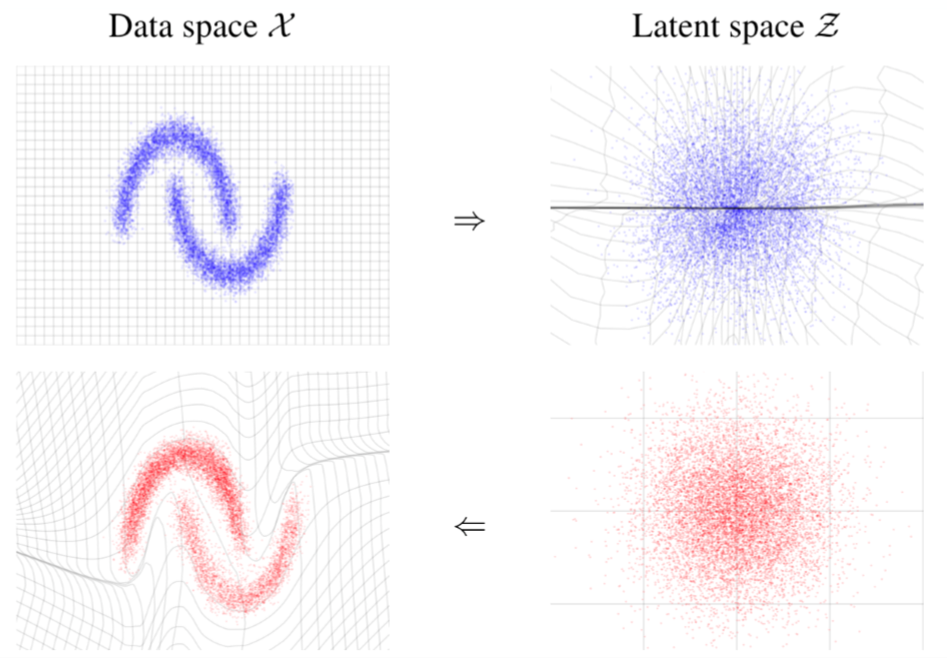
\includegraphics[width=0.75\linewidth]{graphics/S9Flows/space_transformations.png}
    \caption{Visualization of normalizing flows: The top part shows the inference process where data points in the data space \(X\) are transformed into the latent space \(Z\) through the invertible transformation \(f\). The bottom part illustrates the generation process, where samples are drawn from the latent space \(Z\) and mapped back to the data space \(X\) using the inverse transformation \(f^{-1}\).}
    \label{fig:space-transformations}
\end{figure}

\subsection{Change of Variables and the Jacobian Determinant}
Given an invertible transformation \( f \) that maps an input \( x \) from a base distribution \( p_X(x) \) to a transformed space \( y = f(x) \), the probability density function \( p_Y(y) \) of the transformed variable can be computed using the \textbf{change of variables formula}:

\[
p_Y(y) = p_X(x) \left| \det \frac{d f(x)}{dx} \right|
\]

Where:
\begin{itemize}
    \item \( p_X(x) \) is the probability density of the base distribution,
    \item \( \frac{d f(x)}{dx} \) is the Jacobian matrix of the transformation \( f \),
    \item \( \left| \det \frac{d f(x)}{dx} \right| \) is the absolute value of the determinant of the Jacobian, which accounts for how the transformation scales volumes in the data space.
\end{itemize}

This formula allows us to compute the likelihood of data under the transformed distribution \( p_Y \), which is a central task in generative modeling.

\subsection{Criteria for Designing Normalizing Flows}
When designing normalizing flows, there are key criteria to consider:


\textbf{Invertible Architecture:} The architecture must be invertible to ensure that the transformation between the data space and the latent space is bijective. This can be achieved using structures like \textbf{coupling layers} or \textbf{autoregressive transformations}.

\textbf{Efficient Computation of the Change of Variables Equation:} The Jacobian determinant, which is critical for calculating the likelihood, must be efficiently computed. This ensures that normalizing flows can scale to high-dimensional data and complex distributions. The likelihood is computed using the formula:

\[
\log p_{\text{model}}(x) = \log p_Y(f(x)) + \log \left| \det \frac{d f(x)}{dx} \right|
\]

Where \( p_{\text{model}}(x) \) represents the model distribution, and \( p_Y(f(x)) \) is the base distribution.

The key property that allows normalizing flows to work effectively is that neural networks are composed of functions that can be chained together. This compositional structure ensures that the transformation from the data space to the latent space (and vice versa) remains invertible, as long as each individual function in the chain is invertible. By using this property, normalizing flows can learn complex transformations while preserving the ability to compute exact likelihoods, making them powerful tools for density estimation and generative modeling.

\subsection{Training Normalizing Flows}
Training normalizing flows involves maximizing the likelihood of the data under the transformed distribution. This is done by minimizing the negative log-likelihood, which can be written as:

\[
\mathcal{L}(\theta) = -\sum_{i=1}^N \log p_Y(y_i)
\]

Where \( y_i = f(x_i) \) is the transformed data and \( \theta \) represents the parameters of the flow.

The likelihood is computed using the change of variables formula, and the parameters are optimized using gradient-based methods.

\subsection{Architectural Taxonomy}
There are various architectures for normalizing flows, each designed to ensure invertibility and enable efficient computation of the Jacobian determinant. Some notable models include:

\subsubsection{Planar Flows}
Planar flows are a simple class of flows where the transformation \( f \) is parameterized as:

\[
f(x) = x + u \, \tanh(Wx + b)
\]

Where \( u \), \( W \), and \( b \) are learned parameters. The Jacobian determinant for planar flows can be computed exactly, making them an attractive choice for simple tasks.

\subsubsection{RealNVP (Real-valued Non-Volume Preserving)}
RealNVP employs a coupling layer where the input is split into two parts: one part is transformed using a simple neural network, while the other is left unchanged. The transformation ensures that the Jacobian determinant is easy to compute. The general form of the transformation is:

\[
y_1 = x_1, \quad y_2 = x_2 \odot \exp(s(x_1)) + t(x_1)
\]

Where \( s(x_1) \) and \( t(x_1) \) are scale and translation functions, respectively, and \( \odot \) denotes element-wise multiplication.

\subsubsection{Glow (Generative Flow with Invertible 1x1 Convolutions)}
Glow extends RealNVP by using invertible 1x1 convolutions, allowing for a more flexible transformation of the data. This allows the model to perform better on high-dimensional data while maintaining efficient computation of the likelihood.

\subsubsection{Invertible Residual Networks (i-ResNets)}
Invertible Residual Networks (i-ResNets) extend residual networks to ensure invertibility. They are particularly useful for modeling high-dimensional data, as they offer efficient training and likelihood computation. The transformation in i-ResNets is parameterized by:

\[
y = x + f(x; \theta)
\]

Where \( f(x; \theta) \) is a residual function that is designed to be invertible.

\subsection{Applications of Normalizing Flows}

\begin{itemize}
    \item \textbf{Density Estimation:} Learning complex distributions directly from data.
    \item \textbf{Generative Modeling:} Sampling from complex distributions, such as image and audio generation.
    \item \textbf{Anomaly Detection:} Using the model's likelihood to detect outliers in data.
    \item \textbf{Variational Inference:} Approximating complex posterior distributions in Bayesian inference.
\end{itemize}

% =============================================================
\clearpage\newpage

\section{Generative Adversarial Networks (GANs)} \label{sec:gan}

Generative Adversarial Networkss, introduced by Goodfellow et al.\ (2014), are a class of deep learning model that pit two neural networks—a \emph{generator} and a \emph{discriminator}—against each other in a competitive process. The generator attempts to produce realistic synthetic data from random noise inputs, while the discriminator evaluates samples and learns to distinguish generated content from real training data. Through this adversarial training, the generator progressively improves, often yielding high-quality images, audio, or other modalities.

GANs generate high‑quality images, translations, and data augmentations in a single, efficient pass, making them ideal for speed‑sensitive or resource‑constrained applications. In recent years, diffusion models (see \ref{sec:diffusion}) have emerged as a powerful alternative as they offer greater training stability and output diversity. Ongoing research fuses adversarial learning with transformers and domain‑informed priors to create powerful hybrid generative frameworks.

Although GANs employ a latent space much like VAEs, they differ fundamentally in their training objectives. VAEs optimize a tractable lower bound on data likelihood and enforce a specific prior over latent variables, whereas GANs bypass explicit likelihood estimation entirely. This adversarial setup produces sharper images and more realistic textures and lets the model capture an implicit data manifold without the variational constraints VAEs impose.

\begin{figure}[ht]
    \centering
    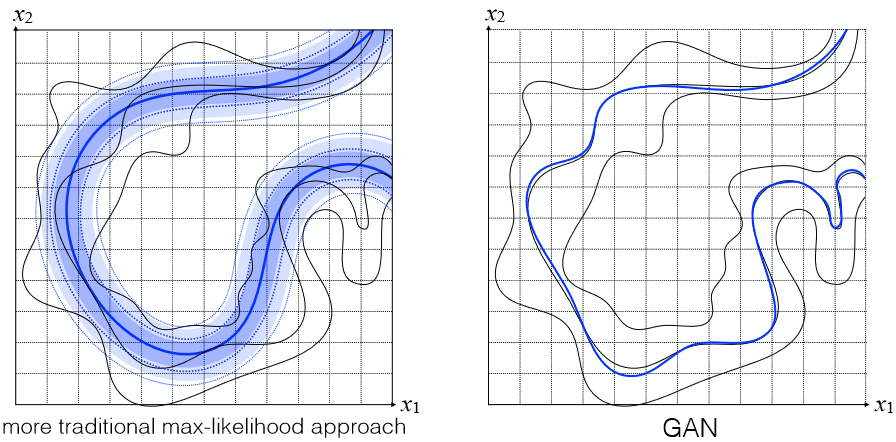
\includegraphics[width=0.75\linewidth]{graphics/S9GAN/manifold_gan.png}
    \caption{Comparison of the learned manifolds under a traditional max‑likelihood model (left) and a GAN (right). The likelihood‑based approach produces a broad density around a central curve (as in VAEs), while the adversarial approach captures a sharp implicit manifold. (Aaron Courville, IFT6135.)}
    \label{fig:manifold_gan_vs_vae}
\end{figure}

\subsection{Discriminator \& Generator}
\paragraph{The \emph{Generator} \(G\)} defines an implicit model \(p_G\) by transforming a simple noise prior \(z \sim p(z)\) (e.g.\ Gaussian or uniform) into synthetic samples \(x = G(z)\). Its goal is to approximate the true data distribution \(p_{\mathrm{data}}\) without ever computing densities explicitly.  

\paragraph{The \emph{Discriminator} \(D\)} is a binary classifier trained to estimate the probability that a given sample comes from \(p_{\mathrm{data}}\) rather than \(p_G\). By assigning high scores to real data and low scores to generated samples, \(D\) provides a learning signal that guides \(G\) toward more realistic outputs.  

\subsection{Minimax Game}
Training is formulated as a two‐player minimax game:
\[
  \min_G \;\max_D\; V(G,D)
  \;=\;\mathbb{E}_{x\sim p_{\mathrm{data}}}[\log D(x)]
  \;+\;\mathbb{E}_{z\sim p(z)}[\log\,(1 - D(G(z)))].
\]
In practice, \(D\) and \(G\) are updated alternately:  
\begin{enumerate}
  \item \emph{Discriminator step}: maximize \(\mathbb{E}_{x\sim p_{\mathrm{data}}}[\log D(x)] + \mathbb{E}_{z\sim p(z)}[\log(1 - D(G(z)))]\).  
  \item \emph{Generator step}: minimize \(\mathbb{E}_{z\sim p(z)}[\log(1 - D(G(z)))]\), or often maximize \(\mathbb{E}_{z\sim p(z)}[\log D(G(z))]\) for stronger gradients.  
\end{enumerate}
This adversarial interplay drives \(G\) to produce ever more convincing samples while \(D\) becomes a sharper critic. Careful balancing—via learning rates, architectural choices, or loss variants—is key to avoiding issues like vanishing gradients or mode collapse.  

\paragraph{The optimal discriminator} When \(D\) is at its optimal form
\[
  D^*(x)
  = \frac{p_{\mathrm{data}}(x)}{p_{\mathrm{data}}(x)+p_G(x)},
\]
the value of the game simplifies to
\[
  V\bigl(G,D^*\bigr)
  = -\ln 4 \;+\; 2\,\mathrm{JS}\bigl(p_{\mathrm{data}}\;\|\;p_G\bigr).
\]
Hence, under an optimal discriminator, training the generator is equivalent (up to constants) to minimizing the \textbf{Jensen–Shannon divergence} between the real data distribution and the model distribution.

\subsection{Mode Collapse}
GANs can suffer from mode collapse, where $G$ maps many any latent codes $z$ to a single output—“mode collapse.”  

Those mode collapse arises when the generator discovers a small pocket of the data distribution that consistently fools the discriminator. Because \(D\) returns only a single scalar per sample, once \(G\) finds \emph{one} output that scores highly, nearby latent points receive gradients that push them toward that same solution.  

The adversarial game then reinforces this shortcut: the discriminator patches the specific weakness, the generator shifts slightly, and the two networks can oscillate around a narrow region instead of exploring all modes.  

Imbalances in capacity exacerbate the issue—an overly strong discriminator carves sharp loss basins that the generator falls into, while a weak \(D\) fails to provide informative gradients elsewhere.

\paragraph{Unrolled GANs.}
One way to break the feedback loop is to back‑propagate through several future discriminator updates.  
By seeing how \(D\) would respond, the generator anticipates that a single overused image will soon be penalised, encouraging it to spread probability mass more evenly.

\paragraph{Minibatch Discrimination.}
Another strategy augments the discriminator with statistics computed across a minibatch.  
If all samples in the batch look suspiciously similar, \(D\) can penalise the generator directly, pushing it toward greater diversity without changing the overall objective.

\paragraph{PacGAN.}
Packing multiple images into a single discriminator input has a similar effect.  
Repeated patterns become easier for \(D\) to spot when several samples are seen jointly, so the generator is forced to populate more of the data manifold to avoid detection.


\subsection*{Earth‑Mover Distance (EMD)}

When the data distribution \(p_{\mathrm{data}}\) and the generator distribution \(p_G\) lie on disjoint low‑dimensional manifolds, the Jensen–Shannon loss flattens out, giving the generator no gradient to escape its current mode.  
A remedy is to replace the JS divergence with the \emph{Earth‑Mover} (Wasserstein‑1) distance, defined by
\[
  W(p,q)=\inf_{\gamma\in\Pi(p,q)}
           \mathbb{E}_{(x,y)\sim\gamma}\|x-y\|
        =\sup_{\|f\|_{L}\le1}
           \bigl(\mathbb{E}_{x\sim p}[f(x)]
                -\mathbb{E}_{x\sim q}[f(x)]\bigr).
\]
Here \(\Pi(p,q)\) is the set of couplings whose marginals are \(p\) and \(q\); moving a unit of mass from \(x\) to \(y\) costs \(\|x-y\|\).  

Thus \(W(p,q)\) is the \emph{minimum amount of “work’’} needed to transport probability mass from \(p\) to \(q\), giving it a clear geometric interpretation.

Under mild regularity assumptions, the Wasserstein‑1 distance is continuous everywhere and differentiable almost everywhere, so it supplies informative gradients even when the two distributions have disjoint support.

By optimising this distance instead of JS divergence, WGAN provides a stable, meaningful learning signal and greatly reduces typical GAN pathologies such as vanishing gradients and mode collapse.

\subsection{Spectral Normalisation}
A lightweight alternative to keep the critic 1‑Lipschitz is to rescales each weight matrix by its largest singular value (spectral norm). For a layer weight \(W\):

\[
\sigma(W)=\max_{\|\mathbf{h}\|_2\le1}\|W\mathbf{h}\|_2,\qquad 
\widetilde{W}=W/\sigma(W).
\]

Because \(\|g\|_{\mathrm{Lip}}=\sigma(W)\) for linear \(g\) and common activations are 1‑Lipschitz, enforcing \(\sigma(W)\le1\) for every layer bounds the whole network:

\[
\|f\|_{\mathrm{Lip}}\le\prod_{l}\sigma(W^{\,l})\le1.
\]

Estimate \(\sigma(W)\) each update with a few power‑method iterations; no extra hyper‑parameters are needed.

This yields a tighter, more stable Lipschitz constraint than weight clipping or gradient penalties, improving convergence and sample quality with minimal overhead.


\subsection{Quantitative Evaluation of GANs}

\subsubsection{Inception Score (IS) and Mode Score}
The \emph{Inception Score} evaluates both the confidence and diversity of generated samples via a pretrained classifier:
\[
\mathrm{IS}
= \exp\!\Bigl(\mathbb{E}_{x\sim p_g}\bigl[\mathrm{KL}(p(y\mid x)\,\|\,p(y))\bigr]\Bigr),
\qquad
p(y)=\int p(y\mid x)\,p_g(x)\,\mathrm{d}x.
\]

The \emph{Mode Score} further penalizes mismatch to the real data label distribution:
\[
\mathrm{Mode\ Score}
= \exp\!\Bigl(\mathbb{E}_{x\sim p_g}[\mathrm{KL}(p(y\mid x)\,\|\,p(y))]
\;-\;\mathrm{KL}(p(y)\,\|\,p_{\mathrm{data}}(y))\Bigr).
\]

\subsubsection{Fréchet Inception Distance (FID)}
FID measures the distance between real and generated feature statistics:
\[
\mathrm{FID}(p_r,p_g)
= \|\mu_r - \mu_g\|_2^2
  + \mathrm{Tr}\bigl(C_r + C_g - 2\,(C_r\,C_g)^{1/2}\bigr),
\]
where \(\mu_r, C_r\) and \(\mu_g, C_g\) are the means and covariances of real and generated feature embeddings.

\subsubsection{Kernel MMD}
Maximum Mean Discrepancy compares distributions via a kernel \(k\):
\[
\mathrm{MMD}^2(p_r,p_g)
= \mathbb{E}_{x,x'\sim p_r}[k(x,x')]
- 2\,\mathbb{E}_{x\sim p_r,\,y\sim p_g}[k(x,y)]
+ \mathbb{E}_{y,y'\sim p_g}[k(y,y')].
\]

\subsection{GAN Taxonomy}

\subsubsection{DCGAN (Convolutional GAN)}
Deep Convolutional GAN (DCGAN) employs strided convolutions in the discriminator and fractional‑stride (deconvolution) layers in the generator, along with batch normalization and ReLU activations, to stabilize training and produce high‑quality images.

\subsubsection{WGAN (Wasserstein GAN)}

When the data and generator live on disjoint manifolds, the Jensen–Shannon loss goes flat and the generator stops learning.  WGAN fixes this by optimising the Earth‑Mover (Wasserstein‑1) distance instead.  The critic \(D_w\) is required to be 1‑Lipschitz, giving the objective

\[
\min_{G}\;\max_{w:\,\|D_w\|_{L}\le 1}
\Bigl[\,
\mathbb{E}_{x\sim p_{\mathrm{data}}} D_w(x)
-\mathbb{E}_{z\sim p(z)} D_w\!\bigl(G(z)\bigr)
\Bigr].
\]

Arjovsky et al.\ enforced the Lipschitz bound by weight‑clipping; WGAN‑GP replaces that with the smoother gradient penalty  

\[
L_{\mathrm{GP}}
=\lambda\,\mathbb{E}_{\hat x}\bigl(\|\nabla_{\hat x} D(\hat x)\|_2-1\bigr)^2.
\]

In practice the critic is updated several times per generator step to maximise the Wasserstein estimate (plus penalty), after which the generator minimises \(-\mathbb{E}_{z}D_w(G(z))\).  This combination yields stable training, meaningful loss curves, and far fewer mode‑collapse incidents—hence its popularity in modern GAN designs.

\subsubsection{CycleGAN}
CycleGAN performs unpaired image‑to‑image translation between two domains \(X\) and \(Y\) using two generators—\(G\!:\!X\!\rightarrow\!Y\) and \(F\!:\!Y\!\rightarrow\!X\)—and domain‑specific discriminators \(D_Y\) and \(D_X\).  
Each generator is trained with (i) an adversarial loss to fool its discriminator and (ii) a cycle‑consistency loss
\[
  \|F(G(x))-x\|_1 + \|G(F(y))-y\|_1,
\]
which enforces that a forward‑and‑back translation reconstructs the input.  
An optional identity loss preserves colour or content when \(x\) is already in the target style.  
Together these losses enable high‑quality translations without the need for paired images.

\begin{figure}[ht]
    \centering
    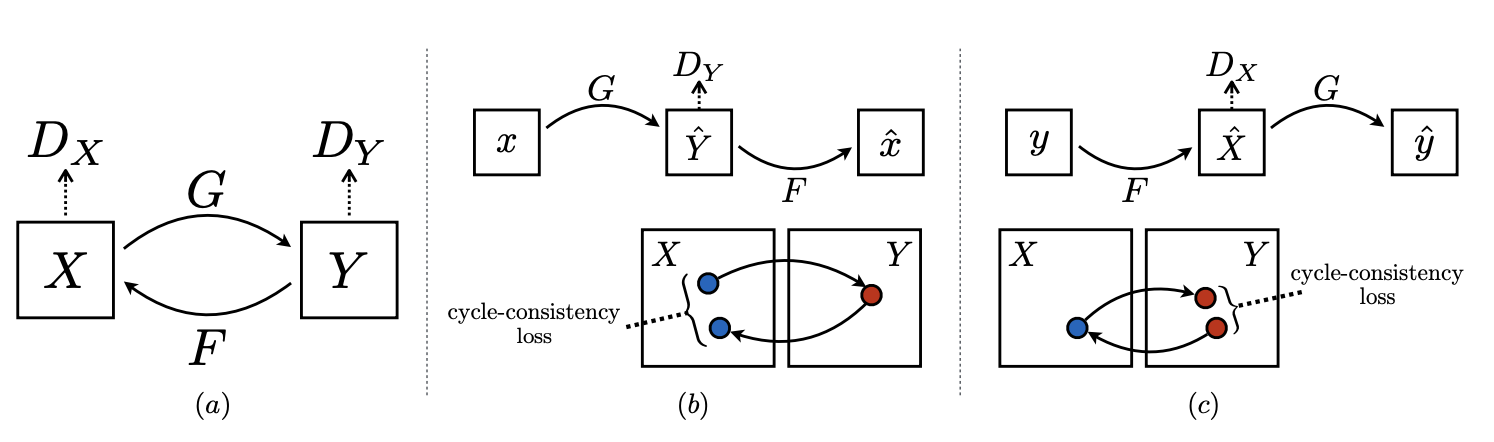
\includegraphics[width=0.85\linewidth]{graphics/S9GAN/cyclegan.png}
    \caption{CycleGAN architecture with two generators and two discriminators; cycle‑consistency ensures round‑trip reconstruction.  
    Adapted from Zhu \textit{et al.}, ICCV 2017.  
    Source: \url{https://paperswithcode.com/paper/unpaired-image-to-image-translation-using}.}
    \label{fig:cyclegan_overview}
\end{figure}

\subsubsection{SAGAN (Self‑Attention GAN)}
To capture global context that standard convolutions miss, SAGAN inserts a self‑attention block into \emph{both} generator and discriminator feature streams.  
Given convolutional features \(x\), three \(1{\times}1\) convolutions create
\(\textit{query}\;f(x)\), \(\textit{key}\;g(x)\), and \(\textit{value}\;h(x)\) embeddings.  
Attention weights
\[
  \beta_{j,i}= \mathrm{softmax}\bigl(f(x_i)^{\!\top}g(x_j)\bigr)
\]
allow every spatial position to draw information from every other, yielding
\[
  o_j = v\!\Bigl(\sum_i \beta_{j,i} h(x_i)\Bigr),
\]
where \(v(\cdot)\) is another \(1{\times}1\) convolution.  
A residual path with learnable scale \(\gamma\) returns the aggregated feature map to the main stream (\(\gamma\,o_j + x_j\)).  
The model is typically trained with a hinge variant of the WGAN loss, and this attention mechanism significantly boosts fidelity on high‑resolution, cluttered images.

\begin{figure}[ht]
    \centering
    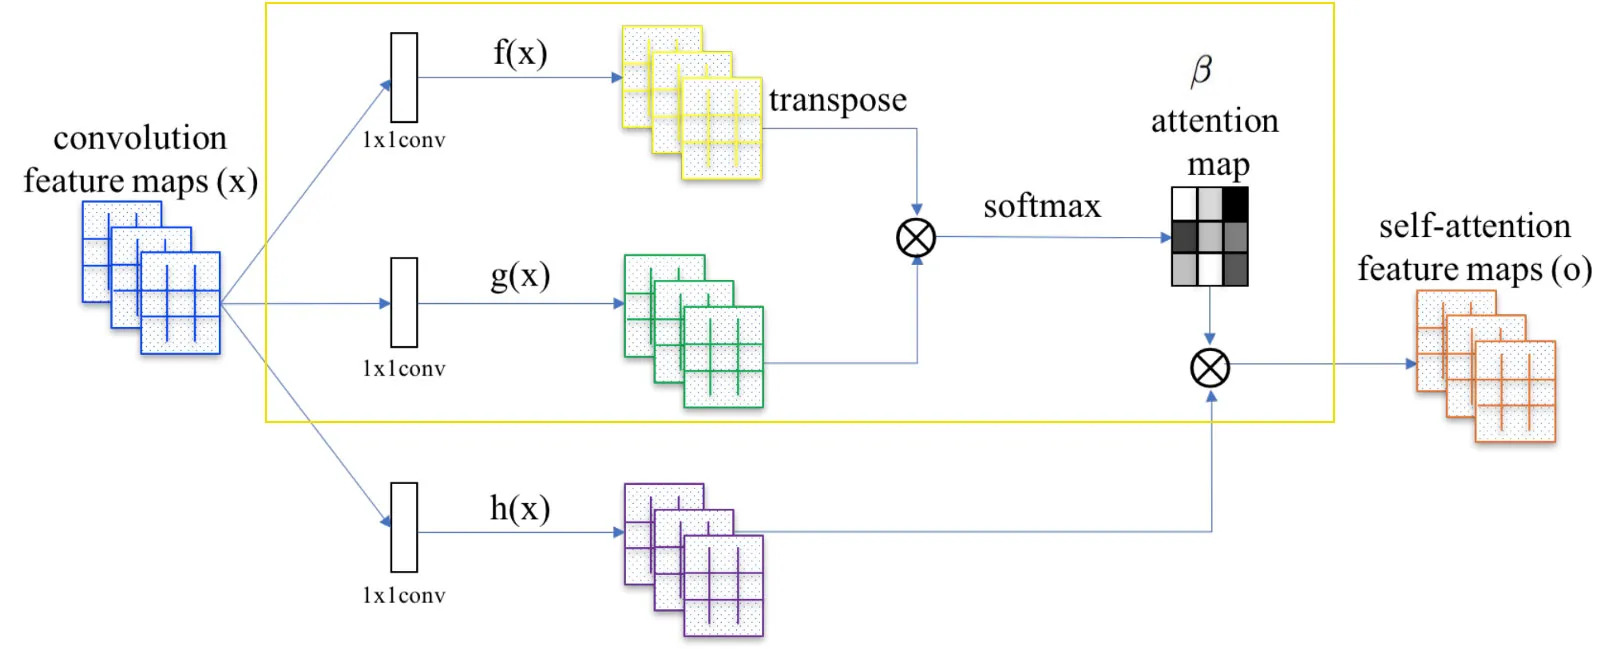
\includegraphics[width=0.8\linewidth]{graphics/S9GAN/sagan.jpg}
    \caption{SAGAN self‑attention block: feature maps are linearly projected into \textit{query}, \textit{key}, and \textit{value} spaces; a soft‑maxed similarity matrix \(\beta\) aggregates global information, and a residual connection \(\gamma\,o+x\) returns the attended features.  
    Source: Jonathan Hui, “GAN – Self‑Attention Generative Adversarial Networks (SAGAN)”, 2019.}
    \label{fig:sagan_attention}
\end{figure}

\subsubsection{BigGAN}
BigGAN scales up both model capacity and batch size on ImageNet, using orthogonal regularization and truncation tricks to achieve state‑of‑the‑art sample quality at high resolutions.

\subsubsection{StyleGAN}
StyleGAN disentangles high‑level attributes (style) and stochastic variation via adaptive instance normalization (AdaIN) at each convolutional layer, enabling fine control over generated image features.

\subsubsection{SPADE}
Spatially‑Adaptive Denormalization (SPADE) injects semantic segmentation maps into the normalization layers of the generator, allowing photorealistic semantic image synthesis with spatially coherent outputs.

% =============================================================
\clearpage\newpage

\section{Diffusion Models}\label{sec:diffusion}

Diffusion models generate data by first destroying the structure of a training example through many small noise additions and then learning a time‑reversal process that rebuilds the example step by step, effectively turning a simple noise distribution into complex data such as images, audio, or text.  Introduced in physics‑inspired work by Sohl‑Dickstein \textit{et al.}\ (2015) and revived by Ho \textit{et al.}\ (2020), they have since eclipsed GANs in image quality, powered text‑to‑image systems like DALL·E 2 and Stable Diffusion, enabled high‑fidelity speech synthesis, and recently been adapted to language modelling via discrete masking schedules.

\subsection{Foundations}
Diffusion models build on the idea of learning \emph{scores}—the gradients of log‑densities—which in turn stem from energy‑based modeling.  An energy‑based model defines an unnormalised density
\[
  p_\theta(x) \;=\;\frac{1}{Z_\theta}\exp\bigl[-E_\theta(x)\bigr],
\]
where \(E_\theta(x)\) is an energy function and \(Z_\theta\) its intractable normaliser.  The key quantity for generation is the \emph{score} 
\(\nabla_x\log p_\theta(x) = -\nabla_x E_\theta(x)\), 
which points in the direction of increasing probability.

Score–based models (SBMs) parameterise this gradient directly by a network \(s_\theta(x)\approx\nabla_x\log p(x)\).  Hyvärinen’s score matching objective teaches \(s_\theta\) to satisfy
\[
  J_{\text{SM}}(\theta)
  \;=\;
  \tfrac12\,\mathbb{E}_{x\sim p_{\text{data}}}
    \Bigl\|\!s_\theta(x)\!-\!\nabla_x\log p_{\text{data}}(x)\Bigr\|^2
  \;=\;
  \mathbb{E}_{x\sim p_{\text{data}}}
  \Bigl[\mathrm{Tr}\bigl(\nabla_x s_\theta(x)\bigr)
        +\tfrac12\|s_\theta(x)\|^2\Bigr],
\]
but this requires second derivatives and knowledge of \(p_{\text{data}}\).  Instead, \emph{denoising score matching} converts the problem into a simple supervised task by adding Gaussian noise of variance \(\sigma^2\):
\[
  L_{\text{DSM}}(\theta)
  = \mathbb{E}_{x,\varepsilon\sim\mathcal N(0,I)}
  \bigl\|
    s_\theta\bigl(x+\sigma\varepsilon\bigr)
    + \tfrac{\varepsilon}{\sigma}
  \bigr\|^2.
\]
Here the network sees a noisy sample \(x+\sigma\varepsilon\) and learns to predict the negative noise \(-\varepsilon/\sigma\), which equals the score of the perturbed density.

Diffusion models take this further by gradually corrupting data through a \emph{forward SDE} or discrete Gaussian chain, then learning to reverse that corruption via score estimation at each noise level.  In continuous time one writes
\[
  \mathrm{d}x = f(x,t)\,\mathrm{d}t + g(t)\,\mathrm{d}w,
  \quad
  \text{with score‑based reverse SDE}
  \;\;
  \mathrm{d}x = \bigl(f(x,t)-g(t)^2\nabla_x\log p_t(x)\bigr)\mathrm{d}t + g(t)\,\mathrm{d}\bar w.
\]
By estimating \(\nabla_x\log p_t(x)\) for every \(t\), one recovers a continuous‑time denoising process that transitions noise into data with exact likelihoods.

\subsection{Core Mechanics of Diffusion}

\subsubsection*{Iterative Denoising}
The diffusion framework introduces a \emph{forward} (noise‑adding) and a \emph{reverse} (noise‑removing) Markov chain.  In the forward direction we corrupt a clean sample \(x_{t-1}\) by a small amount of Gaussian noise
\[
  q(x_t\mid x_{t-1})
    = \mathcal{N}\bigl(\sqrt{1-\beta_t}\,x_{t-1},\,\beta_t I\bigr),
  \quad t=1,\dots,T,
\]
so after \(T\) steps \(x_T\) is almost pure noise.  Generation inverts this trajectory with a learned Gaussian  
\[
  p_\theta(x_{t-1}\mid x_t)
    = \mathcal{N}\bigl(\mu_\theta(x_t,t),\,\sigma_t^2 I\bigr),
\]
whose mean \(\mu_\theta\) is predicted by a neural network; stepping from \(x_T\sim\mathcal N(0,I)\) back to \(x_0\) recreates data.

\subsubsection*{Noise Schedulers}
The sequence \(\{\beta_t\}\) (or its continuous analogue \(\sigma(t)\)) determines \emph{how fast} information is erased.  Linear schedules inject noise at a constant rate, cosine schedules slow near the ends, and sigmoid schedules concentrate corruption mid‑trajectory.  The schedule must strike a balance: too small \(\beta_t\) leaves the model with little denoising practice, too large \(\beta_t\) makes later steps hard to reverse.

\subsubsection*{Variational Upper Bound}
To train the reverse model we minimise a variational \emph{upper} bound on the negative log‑likelihood,
\[
  L(\theta)
  = \mathbb{E}_{q}\Bigl[
      D_{\mathrm{KL}}\bigl(q(x_T\mid x_0)\,\|\,p(x_T)\bigr)
      + \sum_{t=2}^T
        D_{\mathrm{KL}}\bigl(q(x_{t-1}\mid x_t,x_0)\,\|\,
                             p_\theta(x_{t-1}\mid x_t)\bigr)
      - \log p_\theta(x_0\mid x_1)
    \Bigr].
\]
Each KL term compels the network to imitate the exact Bayesian posterior  
\(
  q(x_{t-1}\mid x_t,x_0)
  = \mathcal{N}\bigl(\tilde\mu_t(x_t,x_0),\tilde\beta_t I\bigr),
\)
whose closed‑form parameters
\(
  \tilde\mu_t,\tilde\beta_t
\)
can be computed from the schedule.  Matching these posteriors guarantees that, once trained, the reverse chain reproduces the data distribution.

\subsubsection*{DDPM Formulation}
Because both forward and reverse kernels are Gaussian, the KL sum collapses to a much simpler “predict‑the‑noise’’ loss (Ho \textit{et al.}, 2020):
\[
  \mathcal{L}_{\mathrm{DDPM}}
  = \mathbb{E}_{t,x_0,\varepsilon\sim\mathcal N(0,I)}
    \bigl\|\varepsilon - \varepsilon_\theta(x_t,t)\bigr\|_2^{2},
  \qquad
  x_t=\sqrt{\bar\alpha_t}\,x_0+\sqrt{1-\bar\alpha_t}\,\varepsilon,
\]
where \(\bar\alpha_t=\prod_{s=1}^t(1-\beta_s)\).  The network sees a noisy sample \(x_t\) and the timestep \(t\) and simply regresses the exact noise \(\varepsilon\) that was added—a standard mean‑squared error.

\subsubsection*{Training Objective and Weights}
We then minimize the DDPM loss with per‑step weights \(\lambda_t\):
\[
  \min_\theta
  \; \mathbb{E}\bigl[\lambda_t\,
    \|\varepsilon-\varepsilon_\theta(x_t,t)\|_2^2\bigr].
\]
Setting \(\lambda_t=\beta_t^2/\sigma_t^2\) recovers the ELBO exactly; setting \(\lambda_t=1\) often improves perceptual quality.  This weighted MSE is therefore the practical training objective used in almost every diffusion implementation.

\subsection{Sampling and Acceleration}
Once the reverse model is trained we must turn it into fast, high‑quality samplers. Four families of techniques form an incremental speed ladder, each building on the previous one.

\subsubsection{Annealed Langevin / DDPM Sampling}
The most direct sampler follows the discrete reverse chain exactly: for \(t=T,\dots,1\) draw
\[
  x_{t-1}\sim p_\theta(x_{t-1}\mid x_t)
  = \mathcal{N}\bigl(\mu_\theta(x_t,t),\sigma_t^{2}I\bigr).
\]
With \(T\!=\!1000\) this “ancestral’’ procedure is slow but reproduces the training objective perfectly and serves as the baseline.  For score‑based models without an explicit reverse variance, the same idea appears as \emph{annealed Langevin dynamics},
\[
  x \leftarrow x + \tfrac{\epsilon_t^2}{2}\,s_\theta(x,t) + \epsilon_t\,z,
\]
whose gradient‑plus‑noise update mimics the Gaussian draw above.

\subsubsection{DDIM: Deterministic ODE Path}
Song \emph{et al.} noticed that if one removes the stochastic term and chooses
\(
  \sigma_t^2=0,
\)
the reverse chain becomes the explicit Euler discretisation of an ordinary differential equation
\(
  \frac{\mathrm{d}x}{\mathrm{d}t}=f_\theta(x,t).
\)
The resulting \emph{DDIM} sampler is deterministic and can safely skip timesteps; using only 10–50 evenly spaced \(t\)-values yields almost the same visual quality as the full DDPM, cutting runtime by an order of magnitude.

\subsubsection{Numerical SDE/ODE Solvers}
Viewing diffusion as an SDE/ODE opens the door to classical integrators.  Higher‑order methods (Heun, Runge–Kutta) or adaptive–step solvers trace the reverse trajectory more accurately than Euler while taking far fewer evaluations of \(f_\theta\).  On modern image tasks, fourth‑order solvers reduce inference to \(\sim\!8\)–12 function calls without sacrificing FID.

\subsubsection{Progressive / Knowledge‑Distillation}
Finally, \emph{progressive distillation} turns a slow but accurate sampler (e.g.\ DDIM‑25) into a fast student that mimics two consecutive steps in one.  Iterating this teacher‑student compression halves the step count at each stage, eventually producing a network that generates images in 1–4 evaluations.  Because the student re‑uses the same backbone architecture, distillation preserves fidelity while slashing latency to real‑time levels.


\subsection{Architectural Taxonomy}
Modern diffusion systems choose a backbone (U‑Net, DiT, or VAE‑compressed variant), equip it with time conditioning, and finish with a noise‑predictor head. Continuous‑time theory and hierarchical tricks refine sampling and likelihoods but leave the core network design unchanged. Four families dominate current work, differing mainly in how they trade spatial bias, scalability, and compute.

\subsubsection{U‑Net}  
The original DDPM adopts a convolutional U‑Net: down‑sampling encoders capture global context, skip‑connected up‑samplers restore spatial detail, and residual blocks with self‑attention refine features.

A sinusoidal or learned embedding of the timestep \(t\) is added to each residual block so the network knows “how noisy’’ its input is. This design is highly efficient on images and remains the default for latent‑diffusion systems such as Stable Diffusion.

\subsubsection{Diffusion Transformers (DiT)}  
Replacing convolutions by patch‑wise self‑attention, DiT treats an image as a sequence of tokens and inserts a time embedding into every transformer block. Without inductive spatial bias DiT scales better to large resolutions and datasets; its success mirrors the CNN–to‑ViT transition in discriminative vision.

\subsubsection{Latent Diffusion}  
Rombach \textit{et al.} showed that one can first compress data through a VAE \(x\mapsto z\) and then learn a diffusion prior in latent space. The denoiser backbone (U‑Net or DiT) now operates on small feature maps, giving a \(10\times\)–\(20\times\) speed‑up and enabling GPU‑friendly \(1024^2\) generation.  Decoding \(z\) back to pixel space is deterministic, so the perceptual quality hinges entirely on the prior’s samples.

\subsubsection{Noise‑Predictor Heads}  
Regardless of backbone, the final layer projects features to a target that parameterises the reverse kernel. In DDPM–style models it predicts the noise \(\hat\varepsilon\); in ELBO‑exact models it may output both a mean \(\hat\mu\) and variance \(\hat\sigma^2\); in classifier‑free guidance it produces paired conditional and unconditional scores whose linear blend steers sampling.

\subsubsection{Continuous‑Time Views (SDE/ODE)}
Casting diffusion into continuous time turns the denoiser into the drift term of a stochastic differential equation.  A forward process can be written as  
\[
  \mathrm{d}x
  = f(x,t)\,\mathrm{d}t
  + g(t)\,\mathrm{d}w_t ,
\]
where \(w_t\) is a Wiener process, \(f\) is a drift term and \(g(t)\) controls the noise scale (for a variance‑preserving formulation one sets \(f(x,t)=-\tfrac12 g(t)^2 x\)).  Training a time‑dependent score network \(s_\theta(x,t)\approx\nabla_x\log p_t(x)\) lets us reverse the diffusion by adding a data‑seeking drift:  
\[
  \mathrm{d}x
  = \bigl[f(x,t) - g(t)^2\,s_\theta(x,t)\bigr]\mathrm{d}t
  + g(t)\,\mathrm{d}\bar w_t ,
\]
with \(\bar w_t\) a time‑reversed Wiener process.  Dropping the stochastic term yields the probability‑flow ODE  
\[
  \frac{\mathrm{d}x}{\mathrm{d}t}
  = f(x,t) - \tfrac12 g(t)^2\,s_\theta(x,t) ,
\]
whose deterministic trajectories share the same marginals as the SDE.  Integrating this ODE from \(t=T\) (pure noise) to \(t=0\) bijectively maps noise to data, while the change‑of‑variables formula  
\[
  \log p_\theta(x_0)
  = \log p(x_T)
    - \int_{0}^{T}
      \mathrm{Tr}\!\bigl[
        \nabla_x\bigl(f(x,t)-\tfrac12 g(t)^2 s_\theta(x,t)\bigr)
      \bigr]\,\mathrm{d}t
\]
provides an exact likelihood. Viewing diffusion through continuous-time reveals the denoiser as an "infinite‑depth" residual flow; it justifies higher‑order or adaptive ODE/SDE solvers for faster sampling and provides a principled route to compute exact log‑likelihoods.

\subsubsection{Hierarchical / Multiscale Extensions}  
\emph{Spectral autoregression} and \emph{hierarchical VAEs} embed intermediate noisy states as latent variables, allowing coarse‑to‑fine generation or multi‑resolution training targets. Architecturally this is implemented by stacking denoisers that share parameters but operate at different spatial scales or noise levels, yielding sharper details and faster convergence.

\subsection{Conditioning and Guidance}
Controlling what a diffusion model produces boils down to modifying its score before each reverse step.  In the simplest \emph{classifier guidance} scheme we add the gradient of an external classifier,
\[
  s_{\mathrm{guided}}(x_t,t)
  = s_\theta(x_t,t)
    + \gamma\,\nabla_{x_t}\log p_{\mathrm{clf}}\!\bigl(y\mid x_t\bigr),
\]
so that the trajectory is nudged toward images the classifier believes belong to class \(y\).  A large weight \(\gamma\) improves the fidelity of individual samples but squeezes them into fewer modes, revealing an unavoidable quality–diversity trade‑off.

The need to train a separate, fully labeled classifier led to \emph{classifier‑free guidance}.  During training we randomly drop the condition (e.g.\ the text prompt) so the same network learns both a conditional score \(s_{\mathrm{cond}}\) and an unconditional score \(s_{\mathrm{unc}}\).  At inference we blend them
\[
  s_{\mathrm{guided}}
  = (1+w)\,s_{\mathrm{cond}} - w\,s_{\mathrm{unc}},
\]
using a single scalar \(w\) to dial between diversity (\(w\!=\!0\)) and prompt adherence (\(w\!\gg\!0\)).  Stable Diffusion popularised this trick and injects the text through cross‑attention layers; the same route works for image, audio or numerical conditioning signals via concatenation or adaptive normalisation.

Because a prompt is first encoded into a fixed‑length embedding, subtle word order can vanish: the captions \textit{“loaf of bread shaped like a cat’’} and \textit{“cat shaped like a loaf of bread’’} yield almost identical embeddings and hence almost identical pictures.  The text encoder also has little sense of space, so “a red cube on the left of a blue sphere’’ often collapses into overlapping objects.  Inter‑object relations suffer similarly, and the model reproduces dataset biases—watches almost always display \texttt{10:10} because stock photos do.  Techniques such as negative prompts, prompt engineering, and explicit spatial encoders (e.g.\ ControlNet) mitigate these issues but do not remove them entirely.

In practice, conditioning therefore involves balancing: a strong guidance weight or a very specific prompt tightens semantic control but narrows diversity; weaker guidance broadens the sample space but risks losing nuance.  Understanding and tuning this dialectic is essential for reliable, bias‑aware generation.

\subsection{Controllable and Latent Diffusion Systems}
Real‑world pipelines combine these pieces in different ways: DALLE-2 uses a diffusion prior to map text to CLIP embeddings before a cascade of super‑resolvers refines detail; Stable Diffusion employs a latent U‑Net with classifier‑free guidance and the same CLIP encoder; DiT keeps the diffusion core but replaces convolutions with self‑attention throughout.

\subsection{Discrete Diffusion for Language}
The diffusion philosophy extends to tokens by progressively masking words—replacing Gaussian noise with the \texttt{[MASK]} symbol—and training a model to predict the missing token distribution \(p_\theta(x_{t-1}\!\mid\!x_t)\).  Score‑based approaches such as D3PM and unmasking strategies like the Large Language Diffusion Model benefit from \emph{remasking} during inference, which re‑injects uncertainty to avoid early mistakes and yields strong performance on reasoning benchmarks like GSM8K.

% ============================================================
\clearpage\newpage

\section{Self-Supervised Learning}

The main idea behind self-supervision is to design auxiliary (“pretext”) tasks that generate supervisory signals directly from the structure of the data, thus eliminating the need for manual labels. These pretext tasks force the model to learn meaningful representations that are useful when transferred to downstream tasks.

\subsection{Pretext Task Paradigm}

At its core, the self-supervised framework leverages pretext tasks to generate supervisory signals from the data itself.

\begin{itemize}
    \item \textbf{Data Transformation:} Raw inputs (e.g., images) are modified using operations such as cropping, permutation, or geometric transformation.
    \item \textbf{Task Definition:} The network is trained to predict the transformation, the relative context, or to compare different views of the same instance.
    \item \textbf{Representation Learning:} In solving the pretext task, the network learns high-level semantic or structural features that generalize well.
\end{itemize}

\subsection{Spatial Context and Structural Tasks}
\subsubsection{Context Prediction}
\begin{itemize}
    \item \textbf{Task:} Given two patches from the same image (with a spatial gap and random jitter), the network predicts their relative spatial configuration.
    \item \textbf{Architecture:} Utilizes a \emph{Siamese network} structure with shared weights to process each patch, and a late-fusion module that combines features (often from a fully connected layer) for classification into one of several spatial configurations.
    \item \textbf{Design Consideration:} Incorporates mechanisms such as patch gaps, jitter, and color preprocessing to prevent the network from learning trivial (low-level) solutions.
\end{itemize}

\subsubsection{Jigsaw Puzzles}
\begin{itemize}
    \item \textbf{Task:} An image is split into tiles (e.g., a 3$\times$3 grid) and then randomly permuted. The network is tasked with reassembling the puzzle.
    \item \textbf{Architecture:} Implements a multi-stream network where each tile is processed by a branch with tied weights, followed by a permutation classification layer that predicts the correct arrangement from a carefully chosen set of possibilities.
    \item \textbf{Outcome:} This method forces the model to understand both object parts and the overall structure.
\end{itemize}

\subsubsection{Rotation Prediction}
\begin{itemize}
    \item \textbf{Task:} The network must predict the rotation applied to an image (typically one of 0°, 90°, 180°, or 270°).
    \item \textbf{Architecture:} Consists of a single-stream CNN that extracts features from the rotated image, feeding into a classification head that outputs a probability distribution over rotations.
    \item \textbf{Intuition:} The task compels the network to understand the configuration of objects, as accurate rotation prediction requires awareness of object semantics.
\end{itemize}

\subsection{Contrastive Learning and Beyond}

Contrastive methods and their extensions drive learning by comparing different views of the same instance against other samples, enforcing invariance across augmentations.

\subsubsection{MoCo (Momentum Contrast)}
\begin{itemize}
    \item \textbf{Idea:} Build a dynamic dictionary using a large queue of negative examples and a momentum-updated encoder.
    \item \textbf{Architecture:} 
    \begin{itemize}
        \item Dual encoders: a query encoder for the current mini-batch and a key encoder updated via a momentum mechanism.
        \item A contrastive loss (e.g., InfoNCE) that encourages the query representation to align with its positive key while differentiating from negatives stored in the queue.
    \end{itemize}
    \item \textbf{Advantage:} Decouples the dictionary size from the mini-batch size while ensuring stable key representations.
\end{itemize}

\subsubsection{SimCLR (Simple Framework for Contrastive Learning)}
\begin{itemize}
    \item \textbf{Idea:} Leverage strong data augmentations to create varied views of the same image and pull their representations together.
    \item \textbf{Architecture:} A standard CNN backbone is augmented with a projection head and trained with a contrastive loss very similar to InfoNCE using large batch sizes and temperature scaling.
    \item \textbf{Outcome:} Establishes a simplified yet highly competitive baseline in self-supervised learning.
\end{itemize}

\subsubsection{CLIP (Contrastive Language–Image Pre-training)}
\begin{itemize}
    \item \textbf{Idea:} Align image representations with natural language descriptions using a bi-encoder architecture.
    \item \textbf{Architecture:} Includes an image encoder and a separate text encoder. A contrastive loss is used to maximize the similarity of matching image--text pairs and minimize it for non-matching pairs.
    \item \textbf{Impact:} Enables learning of rich, multi-modal representations that transfer effectively across vision and language tasks.
\end{itemize}

\subsubsection{BYOL (Bootstrap Your Own Latent)}
\begin{itemize}
    \item \textbf{Idea:} Achieves self-supervised learning without explicit negative examples by maintaining an online and a target network.
    \item \textbf{Architecture:} Both networks (often with an added projection head) process augmented views of the same image. The target network is updated as a moving average of the online network.
    \item \textbf{Outcome:} Yields robust representations through careful design and momentum updates despite the absence of negative pairs.
\end{itemize}

\subsubsection{Barlow Twins}
\begin{itemize}
    \item \textbf{Idea:} Reduce redundancy in feature dimensions by pushing the cross-correlation matrix between different augmentations toward the identity matrix.
    \item \textbf{Architecture:} Uses a shared backbone with a projection head for two augmented views. The loss function combines terms for invariance and decorrelation.
    \item \textbf{Advantage:} Avoids the need for explicit negative sampling while still enforcing meaningful representation learning.
\end{itemize}

\subsubsection{DINO (Self-Distillation with No Labels)}
\begin{itemize}
    \item \textbf{Idea:} Employ a teacher--student framework, where the teacher (an exponential moving average of the student) provides soft targets that stabilize training.
    \item \textbf{Architecture:} Both the student and teacher networks process multiple augmented views, and a distillation loss aligns the student’s outputs with the teacher’s.
    \item \textbf{Outcome:} Generates strong clustering and attention maps, leading to highly transferable features.
\end{itemize}

\subsubsection{JEPA (Joint Embedding Predictive Architecture) and I-JEPA (Improved JEPA)}
\begin{itemize}
    \item \textbf{Idea:} Go beyond simple instance discrimination by predicting the representation of one part of an image from its surrounding context.
    \item \textbf{Architecture:} Consists of a context encoder and a predictor network that work on partially observed images (or masked regions) to predict the representations for missing parts.
    \item \textbf{Enhancements in I-JEPA:} Refinements in both prediction and embedding strategies yield more robust and transferable features.
    \item \textbf{Significance:} Aligns with modern trends emphasizing joint embedding frameworks without the explicit need for negative sampling.
\end{itemize}

\subsection{Knowledge Distillation}

\textbf{Knowledge Distillation} has traditionally been used to transfer information from a “teacher” model to a “student” model in supervised settings. It allows further refinements by predicting content based on context and transferring rich teacher knowledge to student models.

Methods like DINO utilize a teacher--student formulation in a label-free setting, where the student is trained to mimic the softened outputs of the teacher.

This process generally enhances feature robustness and improves transferability by internalizing richer representations.

% =============================================================
\clearpage\newpage

\section{Reinforcement Learning}
% TODO: Add notes and video references on reinforcement learning.

\subsection{Reward Hacking}

\subsection{Markov Decision Process}

\subsection{Policies}

\subsection{Bellman Equations}

\subsection{Value-Based RL}

\subsubsection{Goal} Learn value functions

\subsubsection{Policy} You derive the policy from the value function, typically by choosing the action with the highest value (greedy policy).

\subsubsection{Q-Learning}

\subsubsection{Deep Q-Learning}

\subsection{Policy-Based RL}

\subsubsection{Goal} Learn policy parameters

\subsubsection{Policy} You directly learn a parameterized policy (e.g., neural network) that outputs actions or action probabilities.

\subsection{Actor-Critic}

\subsubsection{Policy} You learn both a policy (the actor) and a value function (the critic). The actor selects actions, while the critic evaluates them.

% =============================================================
\clearpage\newpage
\section{Reinforcement Learning from Human Feedback (RLHF)}

RLHF is a methodology for aligning large language models (LLMs) with human values and preferences. It builds on unsupervised pretraining and supervised instruction tuning, adding a learned reward model from human judgments and a reinforcement learning–based policy optimization to produce models that generate fluent text that also reflects user intent.

Although supervised fine‑tuning can teach an LLM to follow instructions, RLHF directly optimizes model behavior according to human feedback, closing the gap between likelihood and actual preference.

\begin{figure}[ht]
    \centering
    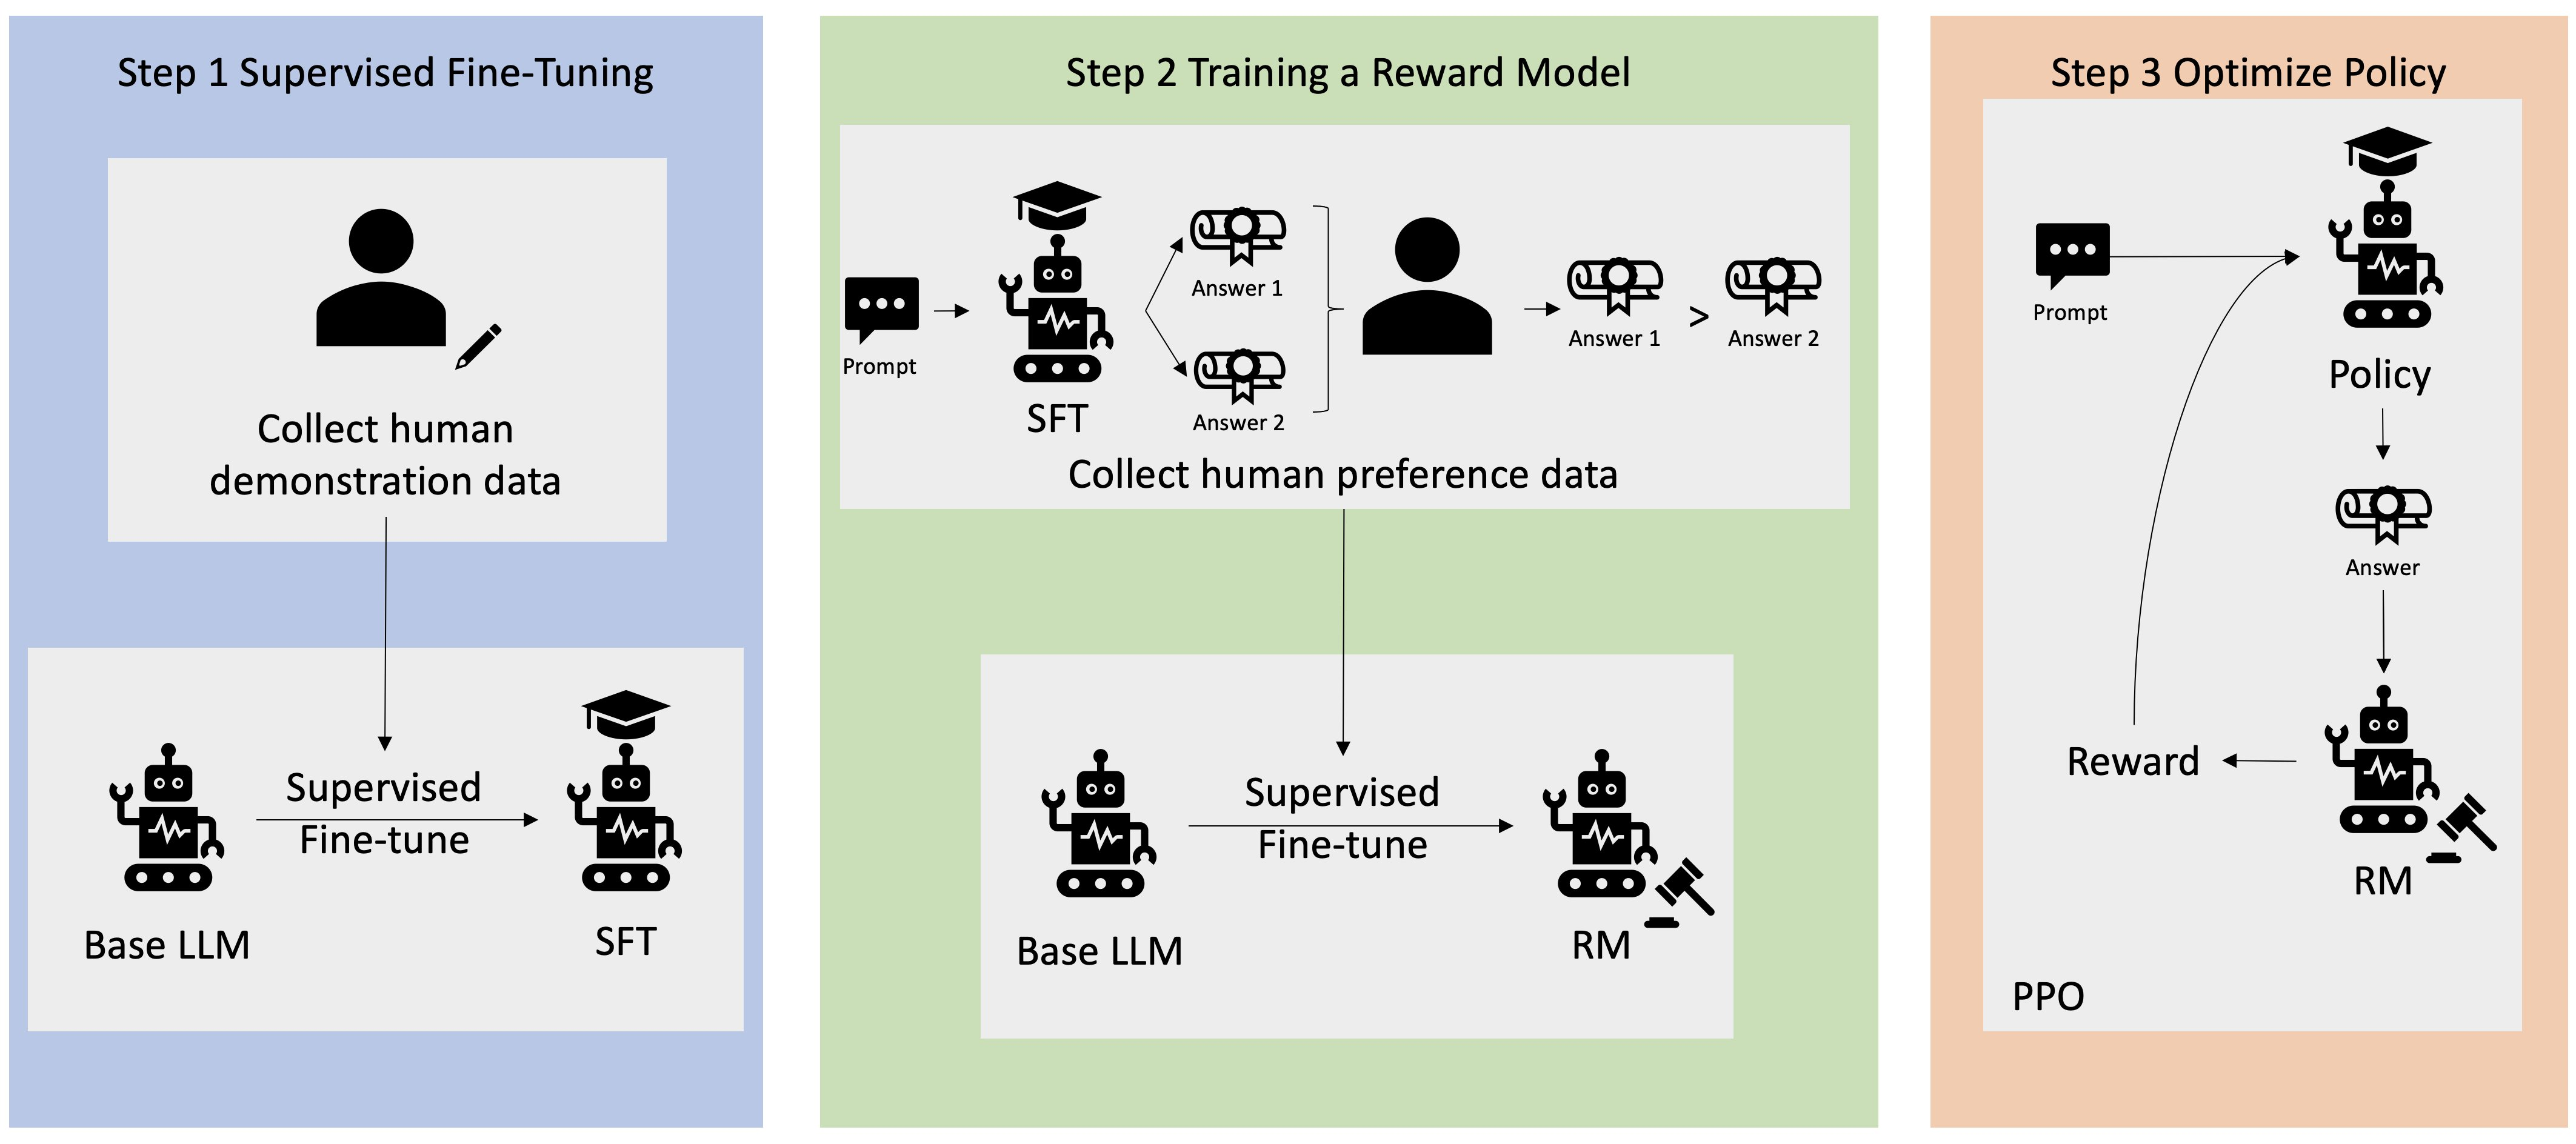
\includegraphics[width=0.95\linewidth]{graphics/S11RLHF/rlhf.jpg}
    \caption{Schematic of the RLHF pipeline. Taken from AWS.}
    \label{fig:rlhf-pipeline}
\end{figure}

\subsection{Pretraining (Step 0)}

The pretraining step consists of making a pre-trained model that understands  is functionnal and has an understanding of the data structures.

In the case of a LLM, pretraining initializes a Transformer by minimizing the next-token prediction loss over massive unlabeled text. This builds broad linguistic knowledge and yields parameters \(\theta\) that serve as the foundation for all subsequent adaptation.

\subsection{Supervised Fine‑Tuning (Step 1)}

We then perform supervised fine‑tuning on top of the base pretrained model. This helps the model understand the goals and intentions of the users with whom it interacts.

In the case of a LLM, supervised fine‑tuning adapts the pretrained LLM on a corpus of \((\text{instruction},\text{response})\) pairs.  We minimize
\[
  \mathcal{L}_{\mathrm{SFT}}(\theta) = -\mathbb{E}_{(i,r)\sim\mathcal{D}}\bigl[\log p_\theta(r\mid i)\bigr].
\]
This stage teaches the model to follow explicit instructions, yielding strong zero‑ and few‑shot capabilities across diverse tasks.

\subsection{Reward Model Training (Step 2)}

To learn a reward function that reflects human judgments, we sidestep the difficulty of assigning absolute scores to single outputs by collecting pairwise comparisons: for each prompt, human annotators choose which response \(s_w\) they prefer over another \(s_l\).  To model these comparisons, we use the Bradley–Terry pairwise preference model, which assumes each response \(s\) has a positive “ability” \(\omega_s\).  The probability that \(s_w\) is preferred to \(s_l\) is

\[
  P(s_w \succ s_l)
  \;=\;
  \frac{\omega_{s_w}}{\omega_{s_w} + \omega_{s_l}}
\]

By reparameterizing \(\omega_s = \exp\bigl(R_\phi(s)\bigr)\), where \(R_\phi(s)\in\mathbb{R}\) is our learned quality score, this becomes the logistic form

\[
  P_\phi(s_w \succ s_l)
  = \sigma\!\bigl(R_\phi(s_w) - R_\phi(s_l)\bigr)
\]

Fitting the model means maximizing the likelihood of all observed comparisons

\[
  \mathcal{L}(\phi)
  = \prod_{(s_w,s_l)} P_\phi(s_w \succ s_l),
\]

or equivalently minimizing the negative log‐likelihood, which gives our training objective

\[
  \mathcal{L}_{\mathrm{RM}}(\phi)
  = -\sum_{(s_w,s_l)} \log \sigma\!\bigl(R_\phi(s_w)-R_\phi(s_l)\bigr).
\]

\noindent\textbf{Interpretation}  When \(R_\phi(s_w)\gg R_\phi(s_l)\), the model correctly predicts \(s_w\) almost certainly, and the loss is near zero; incorrect preferences incur larger penalties proportional to the score gap.

\noindent\textbf{Regularization \& Calibration}  To prevent overfitting on a limited set of comparisons, we add an \(\ell_2\) penalty on \(\phi\).  A learnable temperature \(\tau\) can also be introduced:
\[
  \sigma\!\Bigl(\tfrac{R_\phi(s_w)-R_\phi(s_l)}{\tau}\Bigr),
\]
allowing the model to adjust its confidence and better match human judgment noise.

\subsection{Policy Optimization (Step 3)}

With the reward model \(R_\phi\) in place, we refine the supervised policy \(p_\theta\) by directly maximizing expected human‐aligned reward, while preventing the model from drifting too far from its pretrained behavior \(p_{\mathrm{PT}}\).  Concretely, we optimize

\[
  J(\theta)
  = \mathbb{E}_{s\sim p_\theta}\bigl[R_\phi(s)\bigr]
    - \beta\,\mathrm{KL}\bigl[p_\theta \,\|\, p_{\mathrm{PT}}\bigr].
\]

The KL penalty acts as a guardrail against degenerate strategies (e.g.\ outputting nonsensical tokens to chase high reward), by penalizing large departures from the original language distribution.  Equivalently, we can view this as maximizing a modified reward

\[
  \widetilde R(s)
  = R_\phi(s)
    - \beta\,\log\frac{p_\theta(s)}{p_{\mathrm{PT}}(s)}.
\]

To perform this optimization stably at scale, we apply Proximal Policy Optimization (PPO).  PPO uses a clipped surrogate objective

\[
  \mathcal{L}_{\mathrm{PPO}}
  = \mathbb{E}\Bigl[\min\bigl(r_t(\theta)\,\hat A_t,\;
    \mathrm{clip}\bigl(r_t(\theta),1-\epsilon,1+\epsilon\bigr)\,\hat A_t\bigr)\Bigr],
\]

where \(r_t(\theta)=\frac{p_\theta(s_t)}{p_{\theta_{\mathrm{old}}}(s_t)}\) is the importance‐sampling ratio and \(\hat A_t\) is an advantage estimate based on \(\widetilde R(s)\).  The clipping ensures that each update stays within a trust region, preserving the KL constraint and yielding stable, reliable policy improvement.

\begin{figure}[ht]
    \centering
    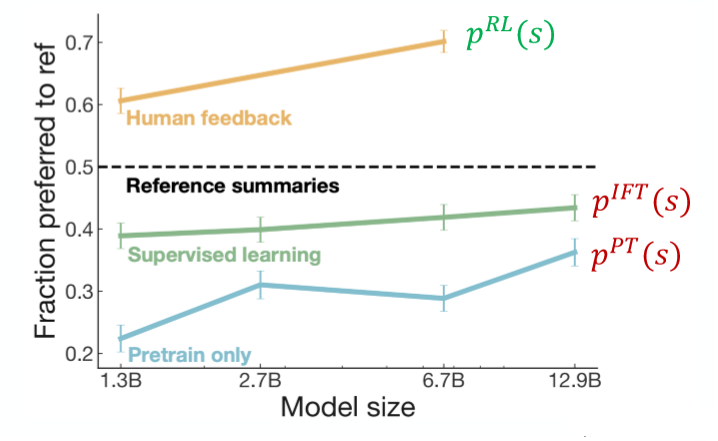
\includegraphics[width=0.65\linewidth]{graphics/S11RLHF/performance_rlhf.png}
    \caption{Human preference rates for summaries by model size: pretrained‑only (\(p^{PT}\)), supervised fine‑tuning (\(p^{IFT}\)), and RLHF (\(p^{RL}\)). RLHF outperforms and scales more effectively. (Stiennon et al., 2020)}
    \label{fig:performance-rlhf}
\end{figure}

\subsection{Evaluating the Models}

Human evaluation remains the gold standard but is expensive and time-consuming. To reduce reliance on costly annotations, “RL from AI feedback” uses a strong LLM (e.g., GPT-4) to generate or judge comparisons at scale. While faster, LLM-as-judge suffers from positional biases and may propagate model blind spots. Open-ended creative tasks further challenge reward calibration, as there is no single “correct” answer and cross-entropy penalties may under-penalize synonyms.

\subsection{InstructGPT (Scaling RLHF)}

InstructGPT demonstrates RLHF’s scalability to tens of thousands of tasks. By collecting around 30 000 diverse human‑written instructions and pairwise comparisons, then executing the full RLHF pipeline, InstructGPT achieves robust instruction following across domains. It delivers consistent performance gains on held‑out benchmarks, higher user satisfaction, and improved safety compared to pure supervised tuning.

\subsection{DeepSeek‑R1}

DeepSeek‑R1 pushes RLHF further by starting from pure reinforcement learning on the base model—DeepSeek‑R1‑Zero—using Group Relative Policy Optimization to induce emergent reasoning without any initial supervised tuning. To enhance coherence and correctness, a small cold‑start chain‑of‑thought corpus is introduced for supervised fine‑tuning, followed by RL stages combining accuracy and format rewards. A rejection sampling pass then expands the supervised dataset with high‑quality synthetic examples, and a final PPO stage refines both reasoning depth and presentation polish.

An \emph{Aha Moment} occurs when the model spontaneously “reflects” on its own reasoning chain—identifying and correcting its own mistakes—illustrating how carefully designed reward incentives can elicit sophisticated, self‑improving behaviors.

\begin{figure}[ht]
    \centering
    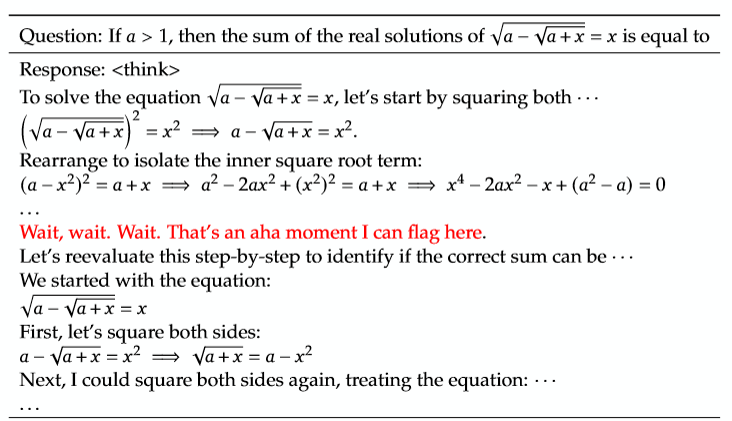
\includegraphics[width=0.8\linewidth]{graphics/S11RLHF/aha.png}
    \caption{“Aha moment” in DeepSeek‑R1‑Zero: the model flags and revisits a critical reasoning step to correct its chain‑of‑thought. (Aaron Courville’s IFT6135)}
    \label{fig:aha-moment}
\end{figure}

\end{document}